{ }%  A simple AAU report template.
%  2015-05-08 v. 1.2.0
%  Copyright 2010-2015 by Jesper Kjær Nielsen <jkn@es.aau.dk>
%
%  This is free software: you can redistribute it and/or modify
%  it under the terms of the GNU General Public License as published by
%  the Free Software Foundation, either version 3 of the License, or
%  (at your option) any later version.
%
%  This is distributed in the hope that it will be useful,
%  but WITHOUT ANY WARRANTY; without even the implied warranty of
%  MERCHANTABILITY or FITNESS FOR A PARTICULAR PURPOSE.  See the
%  GNU General Public License for more details.
%
%  You can find the GNU General Public License at <http://www.gnu.org/licenses/>.
%
%  A simple AAU report template.
%  2015-05-08 v. 1.2.0
%  Copyright 2010-2015 by Jesper Kjær Nielsen <jkn@es.aau.dk>
%
%  This is free software: you can redistribute it and/or modify
%  it under the terms of the GNU General Public License as published by
%  the Free Software Foundation, either version 3 of the License, or
%  (at your option) any later version.
%
%  This is distributed in the hope that it will be useful,
%  but WITHOUT ANY WARRANTY; without even the implied warranty of
%  MERCHANTABILITY or FITNESS FOR A PARTICULAR PURPOSE.  See the
%  GNU General Public License for more details.
%
%  You can find the GNU General Public License at <http://www.gnu.org/licenses/>.
%
\documentclass[12pt,twoside,a4paper,openright]{report}
%%%%%%%%%%%%%%%%%%%%%%%%%%%%%%%%%%%%%%%%%%%%%%%%
% Language, Encoding and Fonts
% http://en.wikibooks.org/wiki/LaTeX/Internationalization
%%%%%%%%%%%%%%%%%%%%%%%%%%%%%%%%%%%%%%%%%%%%%%%%
% Select encoding of your inputs. Depends on
% your operating system and its default input
% encoding. Typically, you should use
%   Linux  : utf8 (most modern Linux distributions)
%            latin1
%   Windows: ansinew
%            latin1 (works in most cases)
%   Mac    : applemac
% Notice that you can manually change the input
% encoding of your files by selecting "save as"
% an select the desired input encoding.
\usepackage[utf8]{inputenc}
% Make latex understand and use the typographic
% rules of the language used in the document.
\usepackage[danish]{babel}
\usepackage[footnote,mode=multiuser,draft,danish,silent,nomargin]{fixme}
% Use the palatino font
\usepackage[sc]{mathpazo}
\linespread{1.35}         % Palatino needs more leading (space between lines)
% Choose the font encoding
\usepackage[T1]{fontenc}
%%%%%%%%%%%%%%%%%%%%%%%%%%%%%%%%%%%%%%%%%%%%%%%%
% Graphics and Tables
% http://en.wikibooks.org/wiki/LaTeX/Importing_Graphics
% http://en.wikibooks.org/wiki/LaTeX/Tables
% http://en.wikibooks.org/wiki/LaTeX/Colors
%%%%%%%%%%%%%%%%%%%%%%%%%%%%%%%%%%%%%%%%%%%%%%%%
% load a colour package
\usepackage{xcolor}
\definecolor{aaublue}{RGB}{33,26,82}% dark blue
% The standard graphics inclusion package
\usepackage{graphicx}
% Set up how figure and table captions are displayed
\usepackage{caption}
\captionsetup{%
  font=footnotesize,% set font size to footnotesize
  labelfont=bf % bold label (e.g., Figure 3.2) font
}
% Make the standard latex tables look so much better
\usepackage{array,booktabs}
% Enable the use of frames around, e.g., theorems
% The framed package is used in the example environment
\usepackage{framed}
\usepackage{adjustbox}   
  

%%%%%%%%%%%%%%%%%%%%%%%%%%%%%%%%%%%%%%%%%%%%%%%%
% Mathematics
% http://en.wikibooks.org/wiki/LaTeX/Mathematics
%%%%%%%%%%%%%%%%%%%%%%%%%%%%%%%%%%%%%%%%%%%%%%%%
% Defines new environments such as equation,
% align and split
\usepackage{amsmath}
% Adds new math symbols
\usepackage{amssymb}
% Use theorems in your document
% The ntheorem package is also used for the example environment
% When using thmmarks, amsmath must be an option as well. Otherwise \eqref doesn't work anymore.
\usepackage[framed,amsmath,thmmarks]{ntheorem}

%%%%%%%%%%%%%%%%%%%%%%%%%%%%%%%%%%%%%%%%%%%%%%%%
% Page Layout
% http://en.wikibooks.org/wiki/LaTeX/Page_Layout
%%%%%%%%%%%%%%%%%%%%%%%%%%%%%%%%%%%%%%%%%%%%%%%%
% Change margins, papersize, etc of the document
\usepackage[
  inner=28mm,% left margin on an odd page
  outer=41mm,% right margin on an odd page
  ]{geometry}
% Modify how \chapter, \section, etc. look
% The titlesec package is very configureable
\usepackage{titlesec}
\titleformat{\chapter}[display]{\normalfont\huge\bfseries}{\chaptertitlename\ \thechapter}{20pt}{\Huge}
\titleformat*{\section}{\normalfont\Large\bfseries}
\titleformat*{\subsection}{\normalfont\large\bfseries}
\titleformat*{\subsubsection}{\normalfont\normalsize\bfseries}
%\titleformat*{\paragraph}{\normalfont\normalsize\bfseries}
%\titleformat*{\subparagraph}{\normalfont\normalsize\bfseries}

% Clear empty pages between chapters
\let\origdoublepage\cleardoublepage
\newcommand{\clearemptydoublepage}{%
  \clearpage
  {\pagestyle{empty}\origdoublepage}%
}
\let\cleardoublepage\clearemptydoublepage

% Change the headers and footers
\usepackage{fancyhdr}
\pagestyle{fancy}
\fancyhf{} %delete everything
\renewcommand{\headrulewidth}{0pt} %remove the horizontal line in the header
\fancyhead[RE]{\small\nouppercase\leftmark} %even page - chapter title
\fancyhead[LO]{\small\nouppercase\rightmark} %uneven page - section title
\fancyhead[LE,RO]{\thepage} %page number on all pages
% Do not stretch the content of a page. Instead,
% insert white space at the bottom of the page
\raggedbottom
% Enable arithmetics with length. Useful when
% typesetting the layout.
\usepackage{calc}

%%%%%%%%%%%%%%%%%%%%%%%%%%%%%%%%%%%%%%%%%%%%%%%%
% Bibliography
% http://en.wikibooks.org/wiki/LaTeX/Bibliography_Management
%%%%%%%%%%%%%%%%%%%%%%%%%%%%%%%%%%%%%%%%%%%%%%%%
\usepackage[backend=biber,
  bibencoding=utf8
  ]{biblatex}
\usepackage{filecontents}
\addbibresource{bib/mybib.bib}

%%%%%%%%%%%%%%%%%%%%%%%%%%%%%%%%%%%%%%%%%%%%%%%%
% Misc
%%%%%%%%%%%%%%%%%%%%%%%%%%%%%%%%%%%%%%%%%%%%%%%%
% Add bibliography and index to the table of
% contents
\usepackage[nottoc]{tocbibind}
% Add the command \pageref{LastPage} which refers to the
% page number of the last page
\usepackage{lastpage}
% Add todo notes in the margin of the document
\usepackage[
%  disable, %turn off todonotes
  colorinlistoftodos, %enable a coloured square in the list of todos
  textwidth=\marginparwidth, %set the width of the todonotes
  textsize=scriptsize, %size of the text in the todonotes
  ]{todonotes}

%%%%%%%%%%%%%%%%%%%%%%%%%%%%%%%%%%%%%%%%%%%%%%%%
% Hyperlinks
% http://en.wikibooks.org/wiki/LaTeX/Hyperlinks
%%%%%%%%%%%%%%%%%%%%%%%%%%%%%%%%%%%%%%%%%%%%%%%%
% Enable hyperlinks and insert info into the pdf
% file. Hypperref should be loaded as one of the
% last packages
\usepackage[T1]{fontenc}
\usepackage{mwe}    % loads »blindtext« and »graphicx«
\usepackage{subfig}



\usepackage{hyperref}
\hypersetup{%
	pdfpagelabels=true,%
	plainpages=false,%
	pdfauthor={Author(s)},%
	pdftitle={Title},%
	pdfsubject={Subject},%
	bookmarksnumbered=true,%
	colorlinks=false,%
	citecolor=black,%
	filecolor=black,%
	linkcolor=black,% you should probably change this to black before printing
	urlcolor=black,%
	pdfstartview=FitH%
}
\usepackage{cleveref} 
% package inclusion and set up of the document
% see, e.g., http://en.wikibooks.org/wiki/LaTeX/Formatting#Hyphenation
% for more information on word hyphenation
\hyphenation{ex-am-ple hy-phen-a-tion short}
\hyphenation{long la-tex}
%
%  A simple AAU report template.
%  2015-05-08 v. 1.2.0
%  Copyright 2010-2015 by Jesper Kjær Nielsen <jkn@es.aau.dk>
%
%  This is free software: you can redistribute it and/or modify
%  it under the terms of the GNU General Public License as published by
%  the Free Software Foundation, either version 3 of the License, or
%  (at your option) any later version.
%
%  This is distributed in the hope that it will be useful,
%  but WITHOUT ANY WARRANTY; without even the implied warranty of
%  MERCHANTABILITY or FITNESS FOR A PARTICULAR PURPOSE.  See the
%  GNU General Public License for more details.
%
%  You can find the GNU General Public License at <http://www.gnu.org/licenses/>.
%
%
%
% see, e.g., http://en.wikibooks.org/wiki/LaTeX/Customizing_LaTeX#New_commands
% for more information on how to create macros

%%%%%%%%%%%%%%%%%%%%%%%%%%%%%%%%%%%%%%%%%%%%%%%%
% Macros for the titlepage
%%%%%%%%%%%%%%%%%%%%%%%%%%%%%%%%%%%%%%%%%%%%%%%%
%Creates the aau titlepage
\newcommand{\aautitlepage}[3]{%
  {
    %set up various length
    \ifx\titlepageleftcolumnwidth\undefined
      \newlength{\titlepageleftcolumnwidth}
      \newlength{\titlepagerightcolumnwidth}
    \fi
    \setlength{\titlepageleftcolumnwidth}{0.5\textwidth-\tabcolsep}
    \setlength{\titlepagerightcolumnwidth}{\textwidth-2\tabcolsep-\titlepageleftcolumnwidth}
    %create title page
    \thispagestyle{empty}
    \noindent%
    \begin{tabular}{@{}ll@{}}
      \parbox{\titlepageleftcolumnwidth}{
        \iflanguage{danish}{%
          
\includegraphics[width=\titlepageleftcolumnwidth]{figures/aau_logo_da}
        }{%
          
\includegraphics[width=\titlepageleftcolumnwidth]{figures/aau_logo_en}
        }
      } &
      \parbox{\titlepagerightcolumnwidth}{\raggedleft\sf\small
        #2
      }\bigskip\\
       #1 &
      \parbox[t]{\titlepagerightcolumnwidth}{%
      \textbf{Abstract:}\bigskip\par
        \fbox{\parbox{\titlepagerightcolumnwidth-2\fboxsep-2\fboxrule}{%
          #3
        }}
      }\\
    \end{tabular}
    \vfill
    \iflanguage{danish}{%
      \noindent{\footnotesize\emph{Rapportens indhold er frit tilgængeligt, men offentliggørelse (med kildeangivelse) må kun ske efter aftale med forfatterne.}}
    }{%
      \noindent{\footnotesize\emph{The content of this report is freely available, but publication (with reference) may only be pursued due to agreement with the author.}}
    }
    \clearpage
  }
}

%Create english project info
\newcommand{\englishprojectinfo}[8]{%
  \parbox[t]{\titlepageleftcolumnwidth}{
    \textbf{Title:}\\ #1\bigskip\par
    \textbf{Theme:}\\ #2\bigskip\par
    \textbf{Project Period:}\\ #3\bigskip\par
    \textbf{Project Group:}\\ #4\bigskip\par
    \textbf{Participant(s):}\\ #5\bigskip\par
    \textbf{Supervisor(s):}\\ #6\bigskip\par
    \textbf{Copies:} #7\bigskip\par
    \textbf{Page Numbers:} \pageref{LastPage}\bigskip\par
    \textbf{Date of Completion:}\\ #8
  }
}

%Create danish project info
\newcommand{\danishprojectinfo}[8]{%
  \parbox[t]{\titlepageleftcolumnwidth}{
    \textbf{Titel:}\\ #1\bigskip\par
    \textbf{Tema:}\\ #2\bigskip\par
    \textbf{Projektperiode:}\\ #3\bigskip\par
    \textbf{Projektgruppe:}\\ #4\bigskip\par
    \textbf{Deltager(e):}\\ #5\bigskip\par
    \textbf{Vejleder(e):}\\ #6\bigskip\par
    \textbf{Oplagstal:} #7\bigskip\par
    \textbf{Sidetal:} \pageref{LastPage}\bigskip\par
    \textbf{Afleveringsdato:}\\ #8
  }
}

%%%%%%%%%%%%%%%%%%%%%%%%%%%%%%%%%%%%%%%%%%%%%%%%
% An example environment
%%%%%%%%%%%%%%%%%%%%%%%%%%%%%%%%%%%%%%%%%%%%%%%%
\theoremheaderfont{\normalfont\bfseries}
\theorembodyfont{\normalfont}
\theoremstyle{break}
\def\theoremframecommand{{\color{gray!50}\vrule width 5pt \hspace{5pt}}}
\newshadedtheorem{exa}{Example}[chapter]
\newenvironment{example}[1]{%
		\begin{exa}[#1]
}{%
		\end{exa}
}
% my new macros

\begin{document}
%frontmatter
\pagestyle{empty} %disable headers and footers
\pagenumbering{roman} %use roman page numbering in the frontmatter
%  A simple AAU report template.
%  2015-05-08 v. 1.2.0
%  Copyright 2010-2015 by Jesper Kjær Nielsen <jkn@es.aau.dk>
%
%  This is free software: you can redistribute it and/or modify
%  it under the terms of the GNU General Public License as published by
%  the Free Software Foundation, either version 3 of the License, or
%  (at your option) any later version.
%
%  This is distributed in the hope that it will be useful,
%  but WITHOUT ANY WARRANTY; without even the implied warranty of
%  MERCHANTABILITY or FITNESS FOR A PARTICULAR PURPOSE.  See the
%  GNU General Public License for more details.
%
%  You can find the GNU General Public License at <http://www.gnu.org/licenses/>.
%
\pdfbookmark[0]{Front page}{label:frontpage}%
%mainfile: ../master.tex
\begin{titlepage}
	\begin{center}
		\newcommand{\HRule}{\rule{\linewidth}{0.5mm}}
		
		% Upper part of the page. The '~' is needed because \\
		% only works if a paragraph has started.
		
\includegraphics[width=0.5\textwidth]{figures/aau_logo_en.pdf}~\\[1cm]
		
		%\textsc{\LARGE Aalborg University}\\[1.5cm]
		
		%\textsc{\Large Project Report}\\[0.5cm]
		
		% Title
		\HRule \\[0.4cm]
		{ \huge NYTORV/ØSTERÅGADE – GÅGADE ELLER BUS-CYKELGADE?\\[0.4cm]
			\large \textsc{P5}}
		
		\HRule \\[1.5cm]
		
		% Author and supervisor
		\begin{minipage}{0.4\textwidth}
			\begin{flushleft} \large
				\emph{Projekt Gruppe}\\
				\textsc{A405a}
			\end{flushleft}
		\end{minipage}
		\begin{minipage}{0.4\textwidth}
			\begin{flushright} \large
				\emph{Vejleder} \\
				\textsc{Katrine Rabjerg Meltofte}
			\end{flushright}
		\end{minipage}
		
		\vfill
		
		% Bottom of the page
		{\large 18. December 2015}
		
	\end{center}
\end{titlepage}

\clearpage

\thispagestyle{empty}
{\small
\strut\vfill % push the content to the bottom of the page
\noindent Copyright \copyright{} Aalborg University 2015\par
\vspace{0.2cm}
\noindent Here you can write something about which tools and software you have used for typesetting the document, running simulations and creating figures. If you do not know what to write, either leave this page blank or have a look at the colophon in some of your books.
}
\clearpage


%\pdfbookmark[0]{English title page}{label:titlepage_en}
%\aautitlepage{%
 % \englishprojectinfo{
  %  Project Title %title
  %}{%
  %  Scientific Theme %theme
  %}{%
   % Fall Semester 2010 %project period
  %}{%
  %  XXX % project group
 % }{%
    %list of group members
   % Author 1\\ 
    %Author 2\\
    %Author 3
  %}{%
    %list of supervisors
   % Supervisor 1\\
    %Supervisor 2
  %}{%
   % 1 % number of printed copies
  %}{%
   % \today % date of completion
 % }%
%}{%department and address
 % \textbf{Electronics and IT}\\
  %Aalborg University\\
 % \href{http://www.aau.dk}{http://www.aau.dk}
%}{% the abstract
 % Here is the abstract
%}

%\cleardoublepage
%{\selectlanguage{danish}
%\pdfbookmark[0]{Danish title page}{label:titlepage_da}
%\aautitlepage{%
  %\danishprojectinfo{
   % Rapportens titel %title
  %}{%
   % Semestertema %theme
  %}{%
   % Efterårssemestret 2015 %project period
  %}{%
   % A405a % project group
 % }{%
    %list of group members
  %  	Abdul Massir Qauomi\\
   % 	Bjørn Carlson\\
    %	Fatimah Daoud\\
    %	Morten Bache Jacobsen\\
    %	Rasmus Steffensen\\
    %	Rong Liu
  %}{%
    %list of supervisors
   % Katrine Rabjerg Meltofte
    
  %}{
    1 % number of printed copies
  %}{%
    \today % date of completion
 % }%
%}{%department and address
  %\textbf{Elektronik og IT}\\
 % Aalborg Universitet\\
  %\href{http://www.aau.dk}{http://www.aau.dk}
%}{% the abstract
 % Her er resuméet
%}}
\markboth{Titlepage}{Titlepage} % Add to header

\begin{nopagebreak}
	{\begin{center}
			\begin{tabular*}{\textwidth}{@{}l@{\extracolsep{\fill}}r@{}}
				\multicolumn{2}{@{}l@{}}{
					\begin{minipage}[t]{1.0\textwidth}
						\vspace{0.3cm}
					\end{minipage}
				}\\
				\begin{minipage}[t]{0.49\textwidth}
					\textbf{Titel}\\
					Nytorv og Østerågade - Trafik konflikter\\
					
					\textbf{Tema}\\
					Virkelighed og modeller indenfor byggeri og anlæg\\
					
					\textbf{Projekt Periode}\\
					Efterårs Semester 2015\\
					
					\textbf{Projekt Gruppe}\\
					A405a\\
					
					\textbf{Forfattere}\\
					Abdul Massir Qauomi\\
					Bjørn Carlson\\
					Fatimah Daoud\\
					Morten Bache Jacobsen\\
					Rasmus Steffensen\\
					Rong Liu\\
					
					\textbf{Vejleder}\\
					Katrine Rabjerg Meltofte\\
					
					\textbf{Kopier}\\
					2\\ % https://www.moodle.aau.dk/course/view.php?id=8838
					
					\textbf{Antal Sider}\\
					\pageref{LastPage}\\
					
				\end{minipage}
				&
				\begin{minipage}[t]{0.49\textwidth}
					\begin{flushright}
						
\includegraphics[height=3cm]{figures/aau_logo_en.pdf}\\
						\small \textbf{Byggeri og Anlæg 1. Semester} \\
						\small \textbf{INSTITUT FOR BYGGERI OG ANLÆG}\\
						\small Badehusvej 13 \\
						\small 9000 Aalborg\\
						\small \url{http://www.byggeri.aau.dk/}\\
						\bigskip
						\fbox{
							\parbox{\linewidth}{
								{\section{Synopsis}
\label{sec:synopsis}
Dette projekt omhandler en tryghedsundersøgelse af trafikken i Nytorv/Østerågade området i Aalborg. Der er set på overvejelser omkring fodgængernes tryghed og sikkerhed i området.
\\\\
Der er blevet redegjort for områdets beliggenhed og struktur, og om begrebet Shared Space. Her er forklaret, hvilke årsager der kan være medvirke til at tiltrække mange trafikanter.
\\\\
Områdets udseende er blevet diskuteret med henblik på Shared Space. Der er herunder set på sammenligninger og folks færden i området.
\\\\
Der er foretaget nogle observationer ved et fodgængerfelt i området, hvor fodgængernes sikkerhed over for cyklisterne er diskuteret. Der er herunder foretaget beregninger af TA-værdien og lavet adfærdsregistrering.
\\\\
Der er lavet interviews af fodgængere, hvor der er set på deres opfattelse af trygheden i området. Herunder er de blevet udarbejdet for at få en forståelse af nogle generelle holdninger og trafikale problemer.
\\\\
Trafiktællinger er blevet foretaget, og der er udarbejdet flow kort over området. Herunder er der lavet beregninger af ÅDT.
\\\\
Forslag til løsninger med henblik på de foretaget observationer, interviews og trafiktællinger er blevet diskuteret og områdets udseende er blevet perspektiveret.

								}
							}}
						\end{flushright}
					\end{minipage}
					
					\\
				\end{tabular*}
			\end{center}
		}
	\end{nopagebreak}

\cleardoublepage
\pdfbookmark[0]{Contents}{label:contents}
\pagestyle{fancy} %enable headers and footers again
\tableofcontents
\listoftodos
%\chapter*{Preface\markboth{Preface}{Preface}}\label{ch:preface}
%\addcontentsline{toc}{chapter}{Preface}
%Here is the preface. You should put your signatures at the end of the preface.

%\vspace{\baselineskip}\hfill Aalborg University, \today
%\vfill\noindent
%\begin{minipage}[b]{0.45\textwidth}
 %\centering
 %\rule{\textwidth}{0.5pt}\\
 % Author 1\\
 %{\footnotesize <username1@XX.aau.dk>}
%\end{minipage}
%\hfill
%\begin{minipage}[b]{0.45\textwidth}
 %\centering
 %\rule{\textwidth}{0.5pt}\\
 % Author 2\\
 %{\footnotesize <username2@XX.aau.dk>}
%\end{minipage}
%\vspace{3\baselineskip}
%\begin{center}
%\begin{minipage}[b]{0.45\textwidth}
 %\centering
 %\rule{\textwidth}{0.5pt}
 % Author 3\\
 %{\footnotesize <username3@XX.aau.dk>}
%\end{minipage}
%\end{center}
%mainfile: ../master.tex
\chapter*{Forord\markboth{Forord}{Forord}}\label{ch:forord}
\addcontentsline{toc}{chapter}{Forord}

Denne rapport er fremkommet ved et samarbejde mellem de 6 gruppemedlemmer i gruppe A405a på Institut for Byggeri og Anlægs første semester på Aalborg universitet. Rapporten er udarbejdet i efterårssemestret 2015. Valget af projektets emne skete på baggrund af, at vi alle i gruppen var enige om, at de trafikale problemer ved Nytorv/Østerågade i Aalborg, var yderst interessante at kigge nærmere på. Rapporten er blevet til i form af gruppearbejde, hvor vi har delt os op to og to, hvor hver minigruppe har fået tildelt et fokusområde i henhold til rapporten. Formålet med rapporten er at belyse de trafikale problemer, som finder sted på Nytorv/Østerågade i Aalborg. Rapporten giver samtidig en mulig løsning på disse problemer. Projektet er skrevet som et led i et byggeteknisk ingeniøruddannelsesprojektforløb.
\\\\
Vi vil gerne benytte lejligheden til at takke vores vejleder Katrine Rabjerg Meltofte for hendes hjælpsomhed, tålmodighed og evne til at inspirere og motivere os. Herudover vil vi gerne takke de mange forbigående fodgængere og cyklister, som har medvirket i vores interviews.
\\\\

\vspace{\baselineskip}\hfill Aalborg Universitet, 18. December 2015
\vfill

\noindent

\begin{minipage}[b]{0.45\textwidth}
	\centering
	\rule{\textwidth}{0.5pt}\\
	Abdul Massir Qauomi\\
	{\footnotesize <aqauom15@student.aau.dk>}
\end{minipage}
%
\hfill
%
\begin{minipage}[b]{0.45\textwidth}
	\centering
	\rule{\textwidth}{0.5pt}\\
	Fatimah Bassam Daoud\\
	{\footnotesize <fdaoud15@student.aau.dk>}
\end{minipage}
%
\vspace{3\baselineskip}

\noindent
\begin{minipage}[b]{0.45\textwidth}
	\centering
	\rule{\textwidth}{0.5pt}\\
	Rasmus Rundh Steffensen\\
	{\footnotesize <rsteff15@student.aau.dk>}
\end{minipage}
%
\hfill
%
\begin{minipage}[b]{0.45\textwidth}
	\centering
	\rule{\textwidth}{0.5pt}\\
	Bjørn Carlson\\
	{\footnotesize <Bcarl15@student.aau.dk>}
\end{minipage}
\vspace{3\baselineskip}

\noindent
\begin{minipage}[b]{0.45\textwidth}
	\centering
	\rule{\textwidth}{0.5pt}\\
	Rong Liu\\
	{\footnotesize <rveste13@student.aau.dk>}
\end{minipage}
%
\hfill
%
\begin{minipage}[b]{0.45\textwidth}
	\centering
	\rule{\textwidth}{0.5pt}\\
	Morten Bache Jacobsen\\
	{\footnotesize <mojaco14@student.aau.dk>}
\end{minipage}
\vspace{3\baselineskip}

\cleardoublepage
%mainmatter
\pagenumbering{arabic} %use arabic page numbering in the mainmatter
\input{sections/report/indledning/indledningmaster.tex}
%mainfile: master.tex
\chapter{Problemformulering}
\label{chap:problemformulering}

%Nytorv/Østerågade er i centrum af Aalborg by. Der er mange moderne butikker, kaffebarer, restauranter og Aalborg`s hovedbibliotek, som giver bosiddende og besøgende et sted at nyde deres fritid. Der er derfor mange mennesker som går ture, shopper, drikker kaffe og spiser sammen med venner i området på Nytorv/Østerågade. Aalborg centrum er et hyggeligt sted at være og med meget leben. Ifølge indledningen kan projektet se, at Aalborgs befolkning stiger. Nytorv/Østerågade er blevet trafiktalt og det har vist sig, at trafikmængden stiger år efter år. Det drejer sig om både busser, cyklister og fodgængere. Der bliver trafikkonflikter med hensyn til shared space.
~\\\\
Det er interresant at se på, hvordan trafikken fungerer nede ved Nytorv/Østerågade området, i og med at der færdes så mange trafikanter, og er et af de centrale steder i Aalborg by. De mange shoppingfaciliteter og cafémuligheder gør det til et attraktivt sted, især for fodgængere, at færde sig i, og derfor er det især denne trafikantgruppe, der er i højsædet i dette projekt. Problemstillingerne er måske ikke så store den dag i dag, men set i perspektivet af, at Aalborg har befolkningsvækst, kan der i fremtiden opstå store trafikale problemer i området. Det er derfor relavent at undersøge, hvilke konflikter, forbigående fodgængere og cyklister mener er til stede mellem dem og de andre trafikantgrupper.
Det er også interresant at se på om området fungerer som et Shared Space område eller noget helt andet.
Det leder efterfølgende til en masse ideer om en eller flere eventuelle løsninger på de trafikale problemer, der kan tænkes at være til stede i området, og dermed løse fremtidens trafikale problemstillinger. Det er især et fokus på en effektivisering af trafik flowet, der i dette projekt cirkuleres omkring. Udgangspunktet i projektet vil blive taget i følgende spørgsmål.
\\\\
Hvilke konflikter finder sted mellem cyklister og fodgængere på Nytorv/Østerågade?
\\
Hvordan kan et løsningsforslag løse de eventuelle konflikter?
\\
Hvordan kan der eventuelt skabes et bedre trafik flow ved området?
\\\\

\section{Afgrænsning}
\label{sec:afgraensning}

I dette projekt er der fokuseret på trafikkonflikter mellem cyklister og fodgængere på Nytorv/Østerågade i Aalborg. Fokuspunktet er fodgængernes tryghed overfor cyklisterne og bilerne. Der vil altså ikke blive fokuseret på buschauførrenes syn på sikkerheden eller dem der kører privatbiler, da de desuden er udelukket fra området. Der er blevet valgt i projektet at afgrænse sig til at lave kvalitative interviews af fodgængere og observationer af Nytorv. Desuden er der en afgrænsning i forhold til de forskellige trafikantgrupper, da der vil blive lavet interviews, udelukkende med forbipasserende som går eller cykler på Nytorv. Der vil blive undersøgt, om fodgængerne føler sig trygge, når de går på Nytorv/Østerågade i Aalborg. Der tages udgangspunkt i konflikter der kan forekomme mellem cyklister og fodgængere, og hvordan man i området kan skabe et bedre trafik flow.

I undersøgelsen har projektet som formål at vurdere disse trafikkonflikter, og ved hjælp af de forskellige observationsmetoder og interviews, komme med et eller flere forslag til nogle konstruktive løsningsforslag som kan forøge trygheden for cyklister samt fodgængere ved Nytorv/Østerågade området.

%master.tex
\chapter{Undersøgelse af trygheden på Nytorv}
\label{chap:undersogelse_af_tryghed}
\section{Analyse og Resultater}
\label{sec:analyseogresult}
Dette afsnit er en undersøgelse af trygheden på Nytorv, som er baseret på observationer af området og interviews af fodgængere. Projektets tilgang til trafikale problemer, vil blive vurderet ud fra disse observationer og interviews. Resultaterne af projektet vil blive præsenteret i dette afsnit, hvoraf der vil blive givet en lille konklusion som afslutning af hver undersøgelse. Afsnittet er altså en sammenkobling af empiri, teori og vurderinger af de forskellige undersøgelser.


\emph{•}\subsection{Shared Space træk i Nytorv/Østerågade området}
\label{omrade_sharedspace}
For at få en forståelse af hvordan trafikanterne færdes i Nytorv/Østerågade området, er det vigtigt først at fastlægge, hvilken type område det er. Området har mange træk fra Shared Space, og derfor er det relevant at sammenligne området med dette begreb.
Tit og ofte anvender man Shared Space i områder, hvor der er et kryds, eller hvor der er et sammenhængende område, for at skabe en slags balance mellem de forskellige trafikantgrupper \autocide{reglershared}.

\begin{figure}[htbp]
   \centering
   \begin{adjustbox}{max width=\textwidth}
     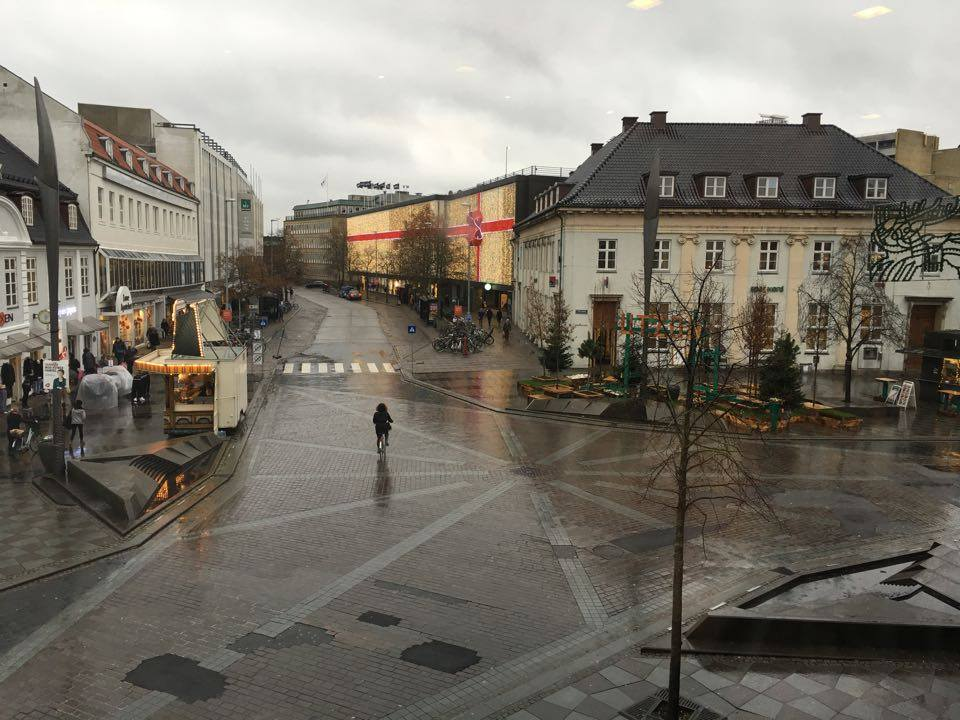
\includegraphics[scale=0.3]{figures/Billederogfigur/Nytorvoverblik.jpg}
  \end{adjustbox}
   \caption{Oveblik over Nytorv}
   \label{fig:nytorv}
 \end{figure}

Med en balance menes der, at et af formålene med et Shared Space er at ingen af trafikantgrupperne vægtes højere end andre trafikantgrupper. På den måde vil man ikke bryde et sammenhængende område, da man forsøger at kombinere hele områdets funktioner i et. Netop dette princip kan man tydeligt fornemme nede ved Nytorv/Østerågade området.  På figur ~\cref{fig:nytorv} side \pageref*{fig:nytorv} 1 kan man se, at området består af et T-kryds, hvor der rundt om er placeret mange shopping faciliteter og caféer. Desuden forbinder området de to gågader, som gør området til et sammenhængende område. Kriterierne for et område, hvor Shared Space kan benyttes, er altså her opfyldt.
Det er tydeligt, at belægningerne, både på fortov og vej, er meget lig udeseende, hvilket er typisk for et Shared Space område \autocide{reglershared}. Der er heller ikke meget afmærkning i form af cykelstier eller kørebaner, som ville have haft til formål at lede trafikanterne. Skiltning, er heller ikke meget brugt og typisk ser man kun et ”E49-, E51- eller E53-skilt” hvilket leder Nytorv/Østerågade området til også at være en sivegade. Skiltene fortæller, at området er en gågade, opholds- og legeområde, eller en fartdæmpet zone, hvor makshastigheden typisk må være 20-30 km/t.  Rundt om Nytorv/Østerågade området, er der skiltet med E53-skilte, hvor der er en tilladt makshastighed på 30 km/t. Det kan ses på figur \cref{fig:Skiltning} side \pageref{fig:Skiltning}, som er taget ved Vindgårdsgade, lige inden gennemgangen fra Boulevarden til Nytorv/Østerågade området. Hvor skiltningerne er, som er illustreret ved de lilla prikker på \cref{fig:midtby} side \pageref{fig:midtby}, er der også skiltet med indkørsel forbudt for privatbiler. 

\begin{figure}[htbp]
   \centering
   \begin{adjustbox}{max width=\textwidth}
     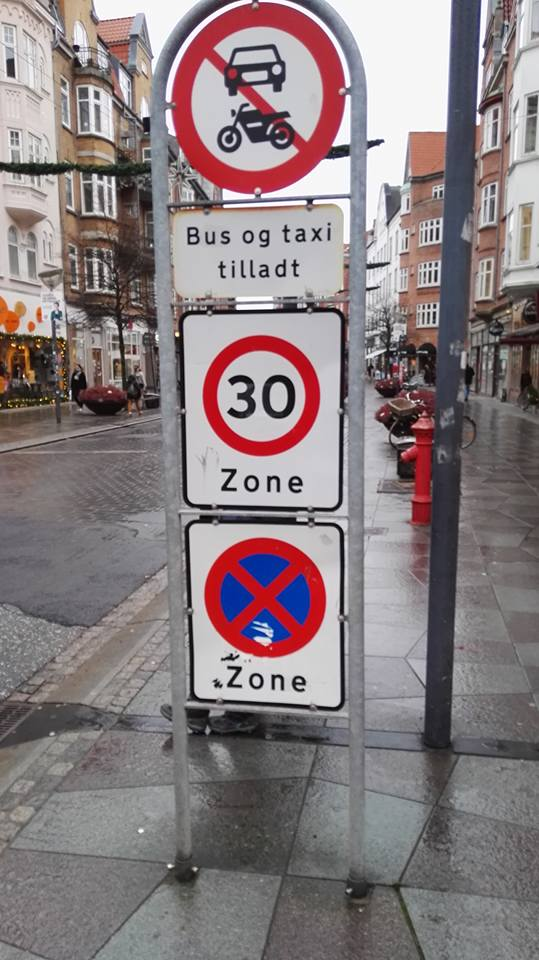
\includegraphics[scale=0.2]{figures/Billederogfigur/skiltning.jpg}
  \end{adjustbox}
   \caption{Skiltning rundt om området}
   \label{fig:Skiltning}
 \end{figure}

I området er der dog en del bustrafik, hvilket strider imod Shared Space’ principper. Det kan give problemer for busserne, at overholde tidsplanerne, da de ofte vil være nødsaget til, at skulle holde tilbage for de mange passerende fodgængere. Det vil derved mindske effektiviteten af den kollektive trafik. Dog er der oftest i ruteplanerne taget højde for en sådan forsinkelse, og på korte strækninger vil indflydelsen kunne tænkes at være begrænset. Busserne kræver nogle busstoppesteder, for at passagerer kan stige af og på busserne i området.

\begin{figure}[htbp]
   \centering
   \begin{adjustbox}{max width=\textwidth}
     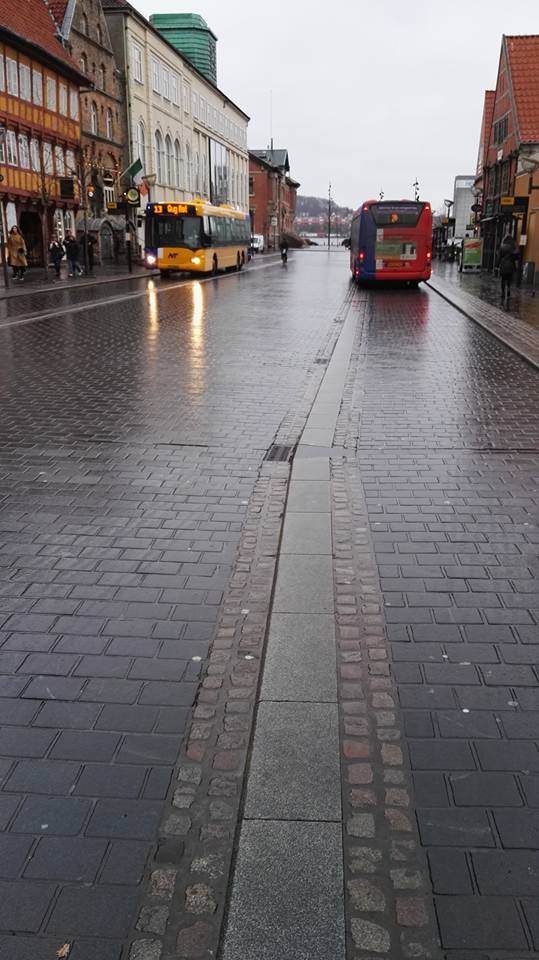
\includegraphics[scale=0.2]{figures/Billederogfigur/Busstoppesteder.jpg}
  \end{adjustbox}
   \caption{De to busstoppesteder}
    \label{fig:Busstoppesteder}
 \end{figure}

På figur \cref{fig:Busstoppesteder} side \pageref{fig:Busstoppesteder} kan man se de to etablerede busstoppesteder, som er placeret lige efter, hvor Bispensgade udmunder ved Østerågade. Placeringen af bustoppestederne er lige udenfor det mest befærdede område, som strækker sig mellem de to gågader og ned ad Nytorv. Det er medvirke til, at det skaber mindst mulige trafikale problemer.
I et Shared Space område kræves også mange holdepladser til cykler. På Nytorv er der på begge sider af vejen et forholdsvist bredt fortov, som har til formål, at skabe en masse plads, hvor cyklerne kan holde parkeret. Det er en nødvendighed, da der færdes mange cykler i området, og for at de mange cyklister skal kunne benytte sig af de mange shopping faciliteter, kræves der altså nogle holdesteder. Et af holdestederne er illustreret på figur \cref{fig:cykelstativ} side \pageref{fig:cykelstativ}.
\begin{figure}[htbp]
   \centering
   \begin{adjustbox}{max width=\textwidth}
     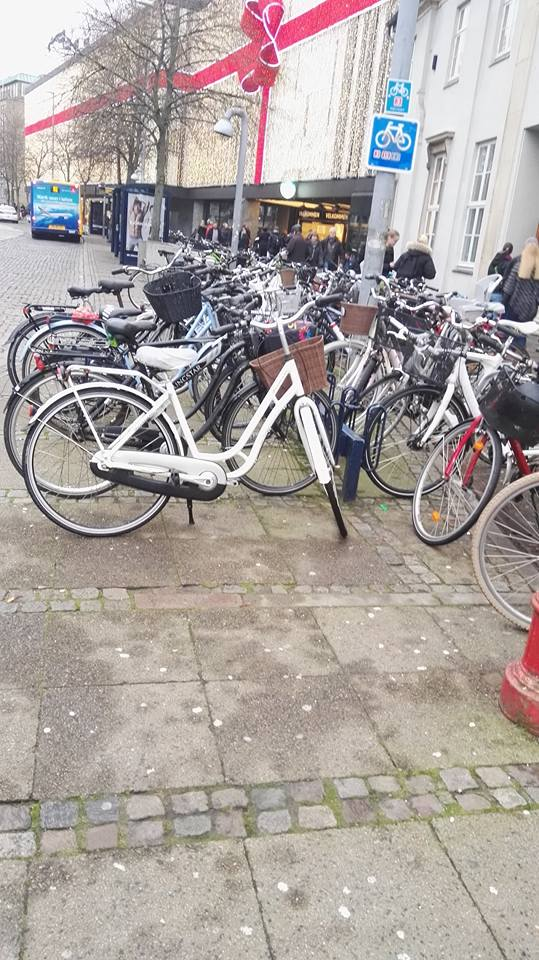
\includegraphics[scale=0.5]{figures/Billederogfigur/cykelstativ.jpg}
  \end{adjustbox}
   \caption{Et af holdepladserne for cykler}
    \label{fig:cykelstativ}
 \end{figure}
Der er altså rigtigt mange træk, som man i området kan observere, minder meget om et Shared Space’ princip, og projektet vil i det næste afsnit undersøge, hvordan området bliver benyttet.


\subsection{Trafikanternes benyttelse af Nytorv som et Shared Space}
\label{benyttelse_omrade}
I området er der meget få retningslinjer og afmærkninger til at lede trafikanterne, hvis stort set ingen. På \cref{fig:Fodfelt} side \pageref{fig:Fodfelt} kan man se en af de to fodgængerfelter, som er i området. Det er på billedet let nok at se afmærkningerne, da billedet er taget fra et fugleperspektiv.

\begin{figure}[htbp]
   \centering
   \begin{adjustbox}{max width=\textwidth}
     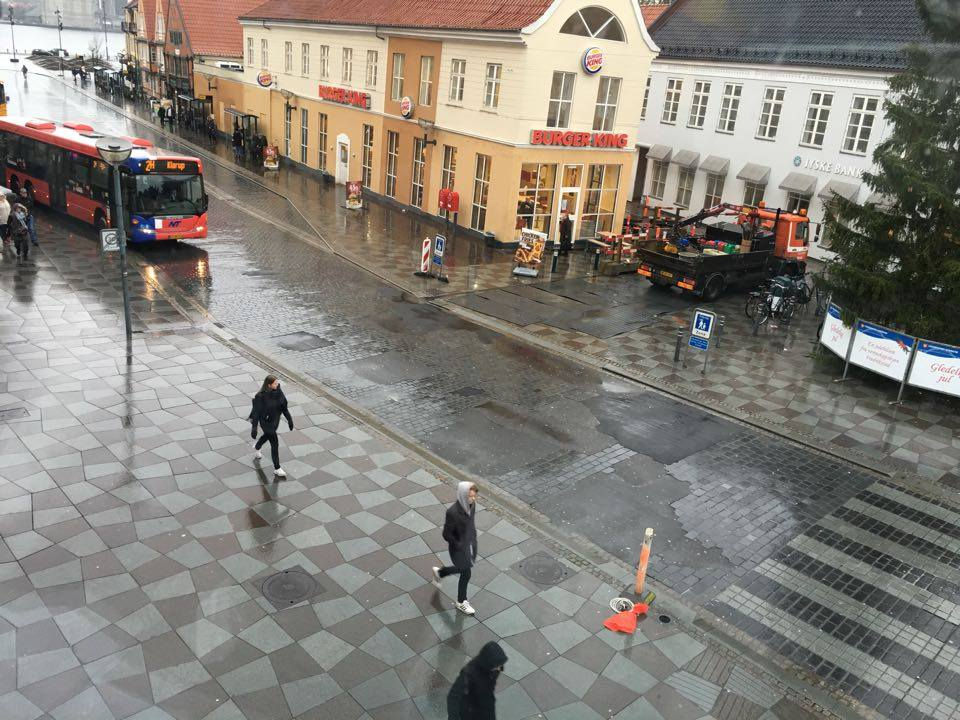
\includegraphics[scale=0.3]{figures/Billederogfigur/Fodfelt.jpg}
  \end{adjustbox}
   \caption{Fodgængeroverfeltet}
   \label{fig:Fodfelt}
 \end{figure}

Men en observation af dette område kan bekræfte, at det kan være svært for cyklisterne at se fodgængerfeltet, når de kommer cyklende mod det. . Det er især cyklister, som kommer rundt svinget fra Nytorv mod havnen. Det er blandt andet også denne hypotese, at interviewsene senere i rapporten tager lidt udgangspunkt i, hvor trygheden for de passerende fodgængere undersøges.
Det er her spørgsmålet kommer ind i billedet, om flere retningslinjer vil skabe mere tryghed. Det er i hvert fald tydeligt, at der er blevet formået at binde området sammen set fra de bløde trafikanters perspektiv. Udelukkelsen af biler har tydeligt præget fordelingen af trafikantgrupper i området, og langt størstedelen er fodgængere og cyklister, hvilket kan aflæses ud fra figur \cref{fig:resultat} og \pageref{fig:resultat}.
En vurdering af området tyder på, at den indbyrdes respekt overfor hinanden, mellem de forskellige trafikantgrupper, ikke er pålagt af området, men individet selv, netop fordi, at området ikke pålægger det. Dette var nogle af de indtryk der blev gjort i de første observationer, som bliver beskrevet under afsnit \cref{sub:foerste_obs} side \pageref{sub:foerste_obs}, på trods af, at der stadig blev observeret nogle konflikter. Shared Space har altså en form for psykologisk effekt, som får trafikanterne til at være opmærksomme på hinanden, og hjælpe hinanden gennem området bedst muligt. Dog er dette ikke et argument for et trygt område at færdes i. Kvalitative interviews vil her være en god måde at undersøge på, om især fodgængerne føler sig trygge, ved at passere området.
I det næste afsnit vil der blive undersøgt via kvalitative interviews, om fodgængerne føler sig trygge overfor cyklisterne, busserne og bilerne, når de passere fodgængeroverfeltet. Herved også for at få en forståelse af, om området føles trygt, og om de Shared Space træk der er i området, skaber trafikale problemer eller ej.

\subsection{Interviews}
Eftersom at fodgængere blev observeret som et problem for cyklisterne, så blev fodgængere også observeret grundigere. Der kan læses mere om observationen i afsnit \ref{sub:foerste_obs}. Der blev identificeret, at fodgængere også var delvis utryg ved Nytorv området, hvilket gav årsag til grundigere undersøgelse, med blandt andet interview med fodgængere.%{XXXXXXX vej.lovportaler.dk} http://vejregler.lovportaler.dk/showdoc.aspx?t=%2fV1%2fNavigation%2fTillidsmandssystemer%2fVejregler%2fAnlaegsplanlaegning%2fTrafikarealer+by%2fVejgeometri+i+byomrader%2f&docId=vd-shared-space-full 10/11-2015}


\subsection{Anvendelse af interviews i praksis}
I denne rapport blev der foretaget et kvalitativt interview med forbigående fodgængere ved Nytorv/Østerågade i Aalborg. Det kvalitative interview leder til kvalitativ viden fra forskellige aspekter, og virker ofte som en metode for, at undersøge nogle bestemte forholde. Under det kvalitative interview bliver interviewpersonerne opfordret til at beskrive hvad de oplever, føler og hvilke ideer og holdninger de har til det givende emne. Derved opnås der under det kvalitative interview konkret viden, i stedet for generelle meninger, som er karakteristisk ved det kvantitative interview. %\footnote{ Hans Reitz Forlag, interview introduktion til et håndværk 2. udgave, side 48}
\\

Herunder kunne et eksempel på en kvalitativ interview være et delvis strukturerede interview, som anvendes, når den teoretisk og praktisk viden er kendt på forhånd, men er åben for nye synsvinkler, holdninger og oplevelser, som interviewpersonerne deler. I forbindelse med interviewet bliver der belyst nogle forholde, som til en vis grad er udarbejdet på forhånd. I rapporten er der en påstand om at det kan føles utrygt, når trafikmiljøet er integreret nede ved Nytorv/Østerågade, herved bruges interviewene blandt andet, som belæg for at det kan virke utrygt, at færdes i området. %\footnote{Ib Andersen, Den skinbarlige virkelighed, side 169}


\subsection{Formålene med interviewene ved Nytorv/Østerågade i Aalborg}
Formålet med interviewet er, at finde initierende problemer og løsninger til, hvordan der kan opnås en effektiv og innovativ sammenbinding af gågade systemet i Aalborg Nytorv/Østerågade. Der blev interviewet fodgængere og cykelister, med hensigten om at de skulle have medbestemmelse i, at skabe en bedre oplevelse af tryghed i området.
\\

I den forbindelse blev der gennemført ca. 20 kvalitative interviews , hvor der blev talte med en forbigående fodgængere og cyklister ad gangen. Interviewene skal bidrage med, at finde løsninger til, hvordan der kan skabes et sikkert og trygt trafikmiljø for alle fodgængere og cyklister.
I værktøjskassen vil der være en række spørgsmål om, hvordan fodgænger og cyklister oplevelser er med at have et integreret trafikmiljø, ønsker ift. hvordan en effektiv sammenbinding af gågadesystemet i Aalborg kunne være, og hvad de tænker om forslaget om løsningerne til problemstillingen i området.
Interviewet er åbent undersøgende om fodgængernes og cyklisterne sikkerhed og tryghed. Der blev afsat 2 timer til interviewet den 14 oktober 2015 fra klokken 13 til 15.%\footnote{https://innovation.blogs.ku.dk/metode/det-kvalitative-interview/ 27/10- 2015}

\subsection{Interview resultaterne med forbigående fodgængere og cyklister ved Nytorv/Østerågade i Aalborg}
 Ud fra de kvalitative interviews (se bilag  cref{chap:interviews}) med forbigående fodgængere og cykelister, resulterede interviewene til, at der var en større enighed om hvorvidt forbipasserende fodgænger og cyklister følte sig utrygge ved at passere Nytorv/Østerågade området i forbindelse med, det integreret trafikmiljø der er. Eksempelvis påstod flere af interviewpersonerne, at de brugte en del tid på at holde øje med om cyklisterne havde set dem. Spørgsmålet lød på om de følte sig trygge ved at gå over fodgængerfeltet, når der færdes mange cyklister ude ved Nytorv/Østerågade i Aalborg, hertil svarede en del,\emph{“Egentlig ikke - jeg synes, at cyklerne kommer meget uventet og meget hurtigt. Jeg holder utroligt meget øje.”} Dette beviser blot at flere fodgængere føler sig utrygge ved at gå over fodgængerfeltet ved området, selvom at de har førsteret til at gå over.
\\

Der er flere årsager, til hvorfor fodgængerene og forbigående cyklister føler sig utrygge i området, eksempelvis mente interviewepersonerne,\emph{”(…), at der kan være kaos herude nogle gange, og det er både cyklister, biler og busser der skaber den kaos.”}. Det vil sige at årsagen til følelsen af utrygheden iblandt fodgængere og forbigående cyklister, delvis er det integreret trafikmiljø der eksisterer, som i visse tilfælde kan udløse et kaos, manglende hensynstagen til andre trafikgrupper, såsom cyklister som ikke holder for fodgængerne ved fodgængerfeltet, mindre kontrol over udelukkelse af privatbiler, da de kan fremføre til større skader, dog er der ingen af interviewpersoner der har oplevet ulykker,  eksempelvis mener en interviewperson, at før vedkommende kan føle sig tryg i trafikken kræver det,\emph{“(…) at busserne og bilerne holder tilbage. Det er dem der kan lave noget skade. Jeg har gået herinde rigtig meget, og jeg har aldrig set en ulykke.”}, selvom at ingen af interviewpersonerne har oplevet en ulykke i området, er tanken om at en større ulykke kan finde sted alligevel skaber utryghed. Derudover skaber den knibende vejplads til cykelister også en utryghed for fodgængerne, eksempelvis påstod en interviewperson, at \emph{“(…) på Boulevarden lagde jeg mærke til at cyklisterne ikke kunne være der, så de måtte trække deres cykler på fortovet (…)".}, da cyklisterne i vissetilfælde trækker deres cykler på fortovet af manglende plads til dem ved Nytorv/Østerågade, skaber det en utryghed for fodgængerne, der går på fortovet.
\\

Der var også en enighed iblandt de forbipasserende fodgængerne og cyklisterne om, at der ønskes en differentiering mellem cyklisterne og kørebanerne. Ønsket lød på, at \emph{“(…) lede cyklerne uden om Nytorv eller dele cyklisterne ud fra kørebanen(…)"}. I og med, hvis ønsket om et differentierede trafikområde blev vedtaget bevæger Nytorv/ Østerågade sig længere væk fra shared space konceptet, hvilket i vissetilfælde vil virke mere trygt for alle trafikantgrupper.
I forbindelse med spørgsmålet om, hvilke ønsker eller forslag de forbigående fodgængere og cykelister havde til at binde gågaden sammen, blev der eksempelvis forslået nogle ønsker om, at \emph{”(…)man kan male fodgængerfeltet hvidt.”}. På nuværende tidspunkt er fodgængerfeltet mellem Bispensgade og Lille Kongensgade grå, en hvid fodgængerfelt frem for den grå, vil virke mere synlig for de kørende og cyklende trafikantgrupper. Nogle interviewpersoner mener også, at mere kontrol over udelukkelse af privatkørsel, en gennemvej for cykelister der skal mod universitet, undergang, overgang eller tunnel vil skabe mere tryghed i området. I den anledning var der også flere ønsker om en køretøjsfrizone, dog var der i højere grad enighed om, at cyklisterne ikke skulle udelukkes fra Nytorv/Østerågade, da nogle synes at de skaber liv i området, og andre påstod at det ikke ville kunne lade sig gøre med den store mængde af cyklister, der cykler til universitet og andre steder hver dag.

%\footnote{Fatimah Daoud,æbleskiver}

\section{Trafiktællinger}
\label{sub:trafiktaellinger}
Dette afsnit tager udgangspunkt i kilden:
\\ http://vej08.vd.dk/mastra/mastradok/dok/TrafiktaellingerPlanUdfoerEfterb.pdf

Trafiktællinger udføres til mange formål. Det gælder alt fra at kontrollere den overordnede vejplanlægning til at undersøge klagesager om for høje trafik hastigheder. Trafiktællinger bruges bl.a. til at finde løsninger til opgaver omhandlende trafiksikkerhed, kapacitet og miljøforhold, samt statistikker over trafikudviklingen og hastigheden af vejnettet. Man kan foretager trafiktællinger manuelt eller ved brug af maskiner.
Manuelle tællinger fungerer ved at personer registrere trafikken på det pågældende sted, ofte ved hjælp af tælleblokke, håndtællere eller håndterminaler. Ved maskine tælling fortages registreringerne automatisk ved brug af et tælleapparat, hvor mennesker ikke medvirker.

\subsection{Manuel tælling}
\label{sub:manuel_taelling}
Manuel tælling er som sagt, hvor det er mennesker der tæller trafikken. Manuel tælling er en god metode, når der ønskes at kende trafikkens specifikke trafikstrømme. Et typisk forløb for manuel tælling er opbygget af 6 trin.
~\\\\
1) Som det første skal formålet for tællingen bestemmes, samt hvilken resultat type, som ønskes af opnå.
~\\\\
Vores formål med trafiktællingen er tælle hvor mange fodgængere, cykelister og billister, som befinder sig inde ved Nytorv og Østerågade. Efterfølgende vil restultaterne blive omregnet  til årsdøgnstrafik ÅDT. Desuden vil der blive noteret hvilken retning trafikanten kom fra og hvilken retning trafikanten begiver sig hen mod. Herved indsamles data, som kan benyttes til at lave et flow kort over trafikken.
~\\\\
2) Der skal besluttes placeringen af tælleposterne, hvor der skal tages hensyn til at tælleren ikke genere trafikken. Tællerne skal også have frit udsyn for parkerende biler, buskaser og lignende under hele tælleperioden. Man skal derfor overveje, om forholdene kan ændre sig undervejs. I trafiktællingen er der observeret ude foran The Harp, som er en bar lige foran fodgængerfeltet på figur \cref{fig:Fodfelt} side \pageref{fig:Fodfelt}, og ligger ud til Østerågade. Her var der et godt overblik over hele området og ingen former for afskærmninger. Herfra blev alle trafikanter og køretøjer noteret.
~\\\\
3) En af de betydlige usikkerheder ved trafiktællinger er valget af tælleperioden. Der kan være meget stor variation fra dag til dag og time til time, hvis der ønskes at finde årsdøgntrafikken. Der er stor forskel på trafikmængden dels i weekenden kontra hverdage og dels i myldretiden om morgen og eftermiddagen kontra midt på dagen og om aftenen og natten. Manuelle tællinger vare typisk 4, 6 eller 12 timer og sjældent et helt døgn. I undersøgelsen er trafiktællingerne lavet en tirsdag d. 24 november kl. 13:00 til 17:00. Det var vurderet til at være de timer på dagen, hvor der færdes flest trafikanter i området. En af ulemperne ved at observere på en tirsdag i området er, at den stor del af de trafikanterne begiver sig rundt i området, for at benytte sig af de mange shoppingfaciliteter og cafeér. Det er især i weekender at folk vil vælge at gøre dette, og derfor ville det være optimalt, at observere en fredag eftermiddag eller en lørdag. Dog er dette bare en af usikkerhederne i vores opregning af årsdøgstrafikken.
~\\\\
4) Når tælleposterne og tidspunkterne er fastlagt, bestemmes antallet af tællere til posterne, vurderet ud fra trafikmængden på det pågældene sted. Ifølge vejdirektoratet er kvaliteten af resultaterne afhængig af antallet af tællere. Er tælleposterne underbemandet, vil resultaterne blive uanvendelige. Hvis man er uvidende om trafikmængden, og dermed antallet af tæller som er nødvendige, kan man foretage en prøvetælling inden. Da Nytorv/Østerågade er et meget befærdet område, er der valgt 6 personer til at tælle. 2 personer observerer køretøjer og cykler ude foran The Herp, 2 personer observerer fodgængere ovenpå McDonalds, og de sidste 2 personer observerer fodgængere ude foran Baresso. (vis dette på kort)
~\\\\
5) Inden tællerne begynder, er det vigtigt at de er sat sig ind i overstående bestemmelser for tælleforløbet, således der ikke opstår tvivler undervejs. Ligeledes udarbejdes et tælleskema inden tællingen påbegyndes. I undersøgelsen er der lavet et tælleskema i Excel, som henholdsvis angiver de forskellige trafikantgrupper og deres retninger. Herefter noteres der for hvert enkelt trafikant, afhængig af trafikantgruppe og retning.
~\\\\
6) Resultatbehandling af tællingen.
\begin{figure}[htbp]
   \centering
   \begin{adjustbox}{max width=\textwidth}
     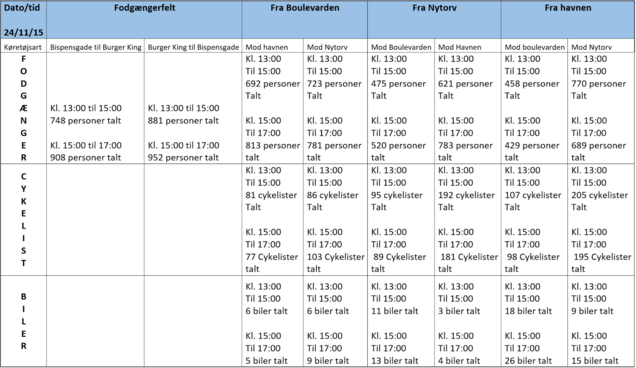
\includegraphics[scale=0.3]{figures/Billederogfigur/resultat.jpg}
  \end{adjustbox}
   \caption{Tabel over trafiktællinger}
   \label{fig:resultat}
 \end{figure}
Der findes ingen omregningsfaktor af fodgængere til ÅDT, derfor er tællingen vurderet, ud fra forholdende på tælledagen. Der blev noteret 2636 fodgængere tirsdag den 24 november kl. 14:00 til 15:00. På dette tidspunkt har skole og gymnasieelever måske fået fri, mens alle som har et 8 til 16 job stadig er på arbejde. Derfor ville der måske have været flere trafikanter, hvis tællingen var lavet senere på den pågældene dag. Til gengæld, hvis tællingerne var taget tidligere og midt i skoletiden, så ville antallet af fodgængere nok være mindre. En anden faktor er, at det regnede mens vi talte. Regnvejret kan have haft en indflydelse på mængden af trafikanter, da det må forventes, at mange vil vælge at benytte sig af området en anden dag. Desuden har dagen og årstiden en stor indflydelse på antallet af fodgængere på Nytorv og Østerågade. Eftersom at der er mange butikker i området, er det ikke bolig– og arbejdetrafik, som benytter sig af området. Det er nærmere folk personlige ærinder eller erhvervstrafikanter. Derfor må det som sagt forventes, at der er flere i weekenderne. I sommerferien vil man også kunne finde meget mere liv, fordi folk mødes, og der bliver afholdt diverse arrangementer nede i byen. Hvis der skal konkluderes på usikkerhederne, er antallet af fodgængere i Østerågade og Nytorv meget situationsafhængig, og resultaterne af trafiktællingerne i rapporten er derfor usikre.
\subsection{Opregning af trafiktællinger til ÅDT}
\label{sub:opregning}
Ved at opregne et antal talte cykler og biler på én dag til ÅDT, vil der altid være en usikkerhed.
I følgende resultatbehandling vil der være fokus på en trafiktælling af cykler og biler ved Nytorv i Aalborg tirsdag d. 24/11 i tidsrummet 13-17. I dette tidsrum er der tale om en blanding af såkaldt bolig/arbejde og by/lokal trafik, da det er i dette tidspunkt, at gennemsnittet af befolkningen får fri fra arbejde og skole, går på indkøb, og i dette tidsrum, at folk skal hjem til sig selv.
Antallet af biler, som vi fik talt i perioden var 104, og antallet af cykler i samme periode var 1408.
For at opregne en trafiktælling, som denne til årsdøgnstrafik, skal man bruge en bestemt formel:
$$ T \times FDT \times FUHDT \times FUDT \times FÅDT = ÅDT $$ eller $$ UDT \times FÅDT = ÅDT$$ , hvor:

$$T = Talt trafik$$

$$UDT = Ugedøgstrafik$$

$$FDT = Opregningsfaktor til døgntrafik i tælleugen$$

$$FUHDT = Opregningsfaktor til ugehverdagsdøgntrafik i tælleugen$$

$$FUDT = Opregningsfaktor til ugedøgntrafik i tælleugen$$

$$FÅDT = Opregningsfaktor til årsdøgntrafik i tælleåret$$

$$FÅR = Opregningsfaktor fra tælleår til andet år$$


\subsection{ÅDT}
\label{AEDT}
\subsubsection{Cyklernes ÅDT på Nytorv i Aalborg}
\begin{figure}[htbp]
   \centering
   \begin{adjustbox}{max width=\textwidth}
     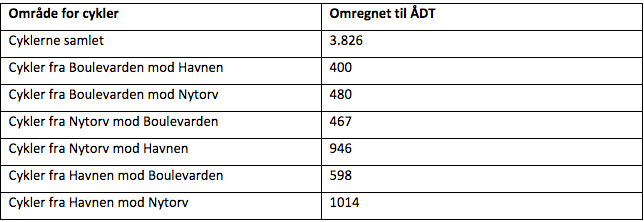
\includegraphics[scale=0.8]{figures/Billederogfigur/cykleradt.jpg}
  \end{adjustbox}
   \caption{Cyklernes ÅDT i Aalborg}
   \label{fig:cykleradt}
 \end{figure}

 \subsubsection{Bilernes ÅDT på Nytorv i Aalborg}
 \begin{figure}[htbp]
   \centering
   \begin{adjustbox}{max width=\textwidth}
     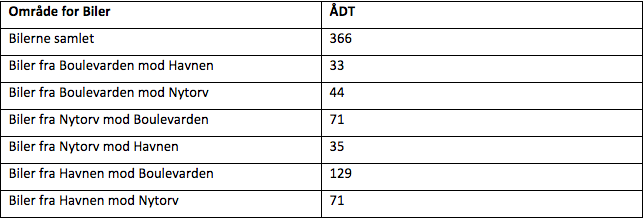
\includegraphics[scale=0.6]{figures/Billederogfigur/bileradt.jpg}
  \end{adjustbox}
   \caption{Bilernes ÅDT i Aalborg}
   \label{fig:bileradt}
 \end{figure}

\subsubsection{Flow kort over biler}
\begin{figure}[htbp]
   \centering
   \begin{adjustbox}{max width=\textwidth}
     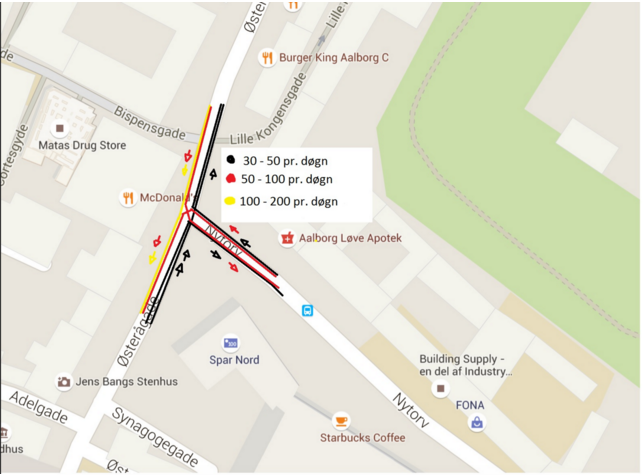
\includegraphics[scale=0.6]{figures/Billederogfigur/bilerflow.jpg}
  \end{adjustbox}
   \caption{Denne illustration viser bilernes flow i løbet af et døgn}
   \label{fig:bilerflow}
 \end{figure}

\subsection{Flow kort over cykler}
\begin{figure}[htbp]
   \centering
   \begin{adjustbox}{max width=\textwidth}
     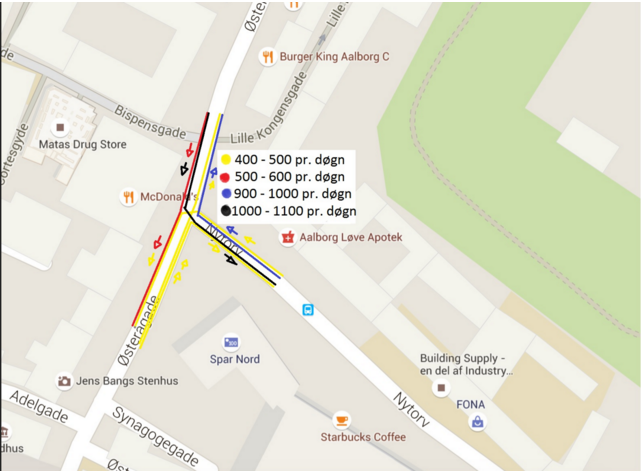
\includegraphics[scale=0.6]{figures/Billederogfigur/cyklerflow.jpg}
  \end{adjustbox}
   \caption{Denne illustration viser cyklernes flow i løbet af et døgn}
   \label{fig:cyklerflow}
 \end{figure}

 \subsection{Flow kort over fodgængere}
 \begin{figure}[htbp]
   \centering
   \begin{adjustbox}{max width=\textwidth}
     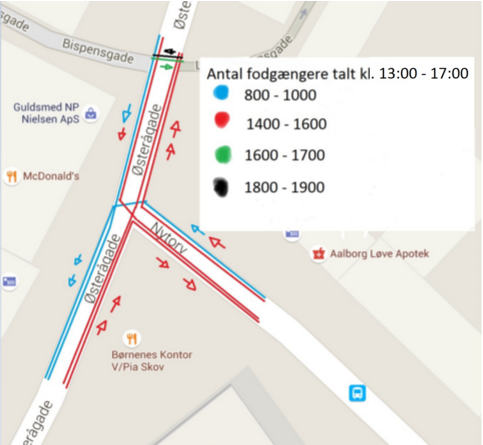
\includegraphics[scale=0.6]{figures/Billederogfigur/fodflow.jpg}
  \end{adjustbox}
   \caption{Denne illustration viser fodgængernes flow i løbet af et døgn}
   \label{fig:fodflow}
 \end{figure}

Resultaterne for de opregnede ÅDT-værdier, som er beregnet ud fra bilag ??, kan ses på ~\cref{fig:cykleradt} og ~\cref{fig:bileradt} side \pageref*{fig:cykleradt}, hjælper os til at give et overblik over, hvor mange antal af hver trafikantgruppe, som bevæger sig i de forskellige retninger. På flowkortet er der givet et mere tydeligt billede af disse tal. Som det kan ses på flowkortet over bilerne, ses det ved hjælp af de farvede afmærkninger, at der er flest biler der passerer området kørende fra havnen mod boulevarden. Ligeledes kan vi se på flowkortet over cyklerne, at ruten, som er mest befærdet er fra havnen op mod nytorv. På det sidste flowkort, kan man se, at der er størst trafik i begge retninger over fodgængeroverfeltet. Hvis man sammenligner de tre flowkort, kan man se, at omkring fodgængeroverfeltet på østerågade, er der flest af alle trafikantgrupper lige netop her. Dette resulterer i, at dette også er stedet, hvor der er størst sandsynlighed for, at en eventuel kollision kan finde sted, da der er flest implicerede parter til stede på samme sted, på samme tid, hver dag.

\subsection{Første observation}
\label{sub:foerste_obs}
Aalborg er byen som arbejder på, at skabe en cykelby.%(http://www.aalborgcykelby.dk/aalborg-cykelby)
Som en cykelby kræver det, at der er en optimal sikkerhed for cyklister blandt andre trafikantgrupper. Trafik flowet ved åbningen af Nytorv blev observeret, området ved McDonalds og Burger King, hvor der kunne ses, at de fleste cyklister havde nogle mindre alvorlige konflikter med bilerne, som krydser Nytorv illegalt. Tværtimod havde cyklisterne lidt større konflikter med fodgængere samt busserne, hvilket også gav et stop for trafik flowet. Derudover kunne der ikke observeres en tryghed på cyklisternes ansigtsudtryk, eftersom de hele tiden skulle være fokuseret og parat til, at bremse ned for fodgængere eller busser. En mindre vurdering kunne bekræfte, at cyklisterne ikke havde en optimal tryghed ved området pga. fodgængere og delvist busserne, eftersom busserne ikke hele tiden krydser Nytorv, men blot hver 5.-6. minut.

Trafik flowet ved slutningen af Nytorv blev observeret, området ved Salling og Friis, her kunne der ses konflikter blandt bilister og cyklister, eftersom cyklisternes cykelsti bliver fjernet. Der kunne tydelig ses en utryghed blandt cyklisterne og bilisterne, da trafikantgrupperne delte vejbanen, hvilket skabte ustruktureret trafikflow ved området og nogle ulovlige overhalinger.

Eftersom fodgængere blev observeret som et problem for cyklisterne, så blev fodgængere også observeret grundigere. Der blev identificeret, at fodgængere også var delvis utryg ved Nytorv området, hvilket gav årsag til grundigere undersøgelse, såsom interview med fodgængere.

\subsection{Dybbere undersøgelse af første observation}
\label{sub:dyb_undersoelse}
I første omgang blev der blot observeret, hvor der blev antaget en række antagelser, hvoraf der til næste observation blev gjort brug af mere specifikke metoder for at identificere trygheden i Nytorv området i Aalborg.
%\\\\
Metoderne bag næste observation var at identificere konflikter ved området. Ved hjælp af konflikterne kan trygheden og sikkerheden for de forskellige trafikantgrupper identificeres. Inden metoderne bliver præsenteret, vil begrebet konflikt blive defineret først. Begrebet konflikt er et meget vidt begreb og dækker indenfor flere fagområder, men i denne rapport bliver begrebet nærmere undersøgt indenfor vej og trafik. Som umiddelbart vil man definere en konflikt, som værende sammenstød mellem to trafikkanter, men dog udelukker den svenske trafikteknik denne påstand.%Kilde
En af metoderne, som bliver anvendt til identificering af konflikterne, er den svenske traftikteknik, hvilket er årsagen til deres definition af konflikt bliver brugt i dette projekt.
%\\\\
Den svenske trafikteknik beskriver en konflikt mellem to trafikkanter, som har kollisionskurs og vil kolligere, hvis en af trafikkanterne ikke foretager sig en pludselig afværgning.2 Det vil sige, at så længe et uheld (sammenstød) kan undgås af mindst en af trafikanterne, så vil der være tale om en konflikt. Ved hjælp af den svenske trafikteknik, kan man dele en konflikt i flere grader. De forskellige konfliktgrader er defineret som alvorlige konflikter, mindre alvorlige konflikter og potentielle konflikter, som også kan ses på \cref{fig:indellingkonflikter} side \pageref{fig:indellingkonflikter}:
 \begin{figure}[htbp]
   \centering
   \begin{adjustbox}{max width=\textwidth}
     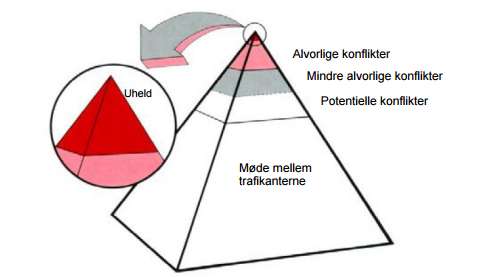
\includegraphics{figures/Billederogfigur/konflikt.png} %http://www.trafitec.dk/sites/default/files/publications/konfliktteknikstudier%20i%20kbh%20bykryds.pdf
  \end{adjustbox}
   \caption{Inddeling af konflikter}
    \label{fig:indellingkonflikter}
 \end{figure}
 \newpage


 En konfliktgrad bestemmes ved hjælp af en TA-værdi. TA-værdien er defineret som tid til ulykke, altså Time to Accident. Metoden bag bestemmelse af TA-værdien gøres ved hjælp af følgende formel:

 $$TU=\frac{d}{V} $$

Hvoraf TA beskriver tid til ulykke \\ d, beskriver distancen til tænkt kollisionspunkt \\ og V, er hastigheden i den undvigeøjeblik.

Formlen fortæller om forholdet mellem distancen til det potentielle punkt i en kollision og hastigheden, når en af trafikanterne undviger uheldet. Heraf kan der ved hjælp af \cref{fig:tagraff} side \pageref{fig:tagraff},
ses om konflikten er alvorlig eller ej.
%~\\\\

\begin{figure}[htbp]

  \centering
  \begin{adjustbox}{max width=\textwidth}
    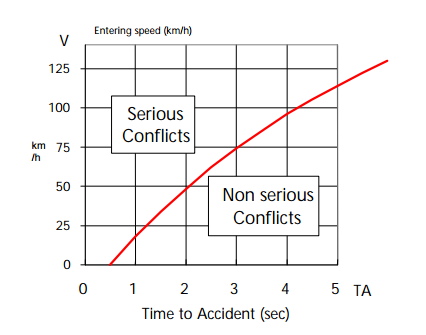
\includegraphics{figures/Billederogfigur/tugraf.png} %http://www.tft.lth.se/fileadmin/tft/video_in_traffic/Swedish_conflict_technique.pdf
 \end{adjustbox}
  \caption{TA-graf}
    \label{fig:tagraff}
\end{figure}

Som der kan ses på %-cref{fig:tagraff}
, så er alvorligheden af en konflikt afhængig af både distance samt hastighed. Dog har hastighed en større rolle i tilfælde af en høj hastighed.
Som udgangspunkt i TA-grafen kan der ses, at en TA-værdi over 0.5 ses som ikke alvorlig konflikt, hvorimod en TA-værdi under ca. 0.5, vil være en alvorlig konflikt.



For at kunne beregne TA-værdien, skal distancen og hastigheden kendes. Distancen og hastigheden kan identificeres ved blot nogle målinger ved området, hvilket i dette projekt blev gjort, som ses på %-cref{fig:maalingerfrabegge}
%\\\\

Som der kan ses på \cref{fig:maalingerfrabegge},
blev området i første omgang målt op fra kanten, som er markeret med farven rød, til fodgængerfeltet og ligeså fra den anden kant, som er markeret med farven blåt. Bemærk de andre markeringer på figuren, som bruges til beregning af TA-værdien, er forskellige længder, altså er d forskellig i formlen for TA-værdien : $$ TU=\frac{d}{V} $$

%\begin{figure}[!ht]
%	\centering
	%\subfloat[First sub-figure\label{subfig-1:obsomrrod}]{\includegraphics[width=1\linewidth]{figures/billederogfigur/rodmarkering.jpg}	}
	%\hfill
	%\subfloat[First sub-figure\label{subfig-2:dummy}]{%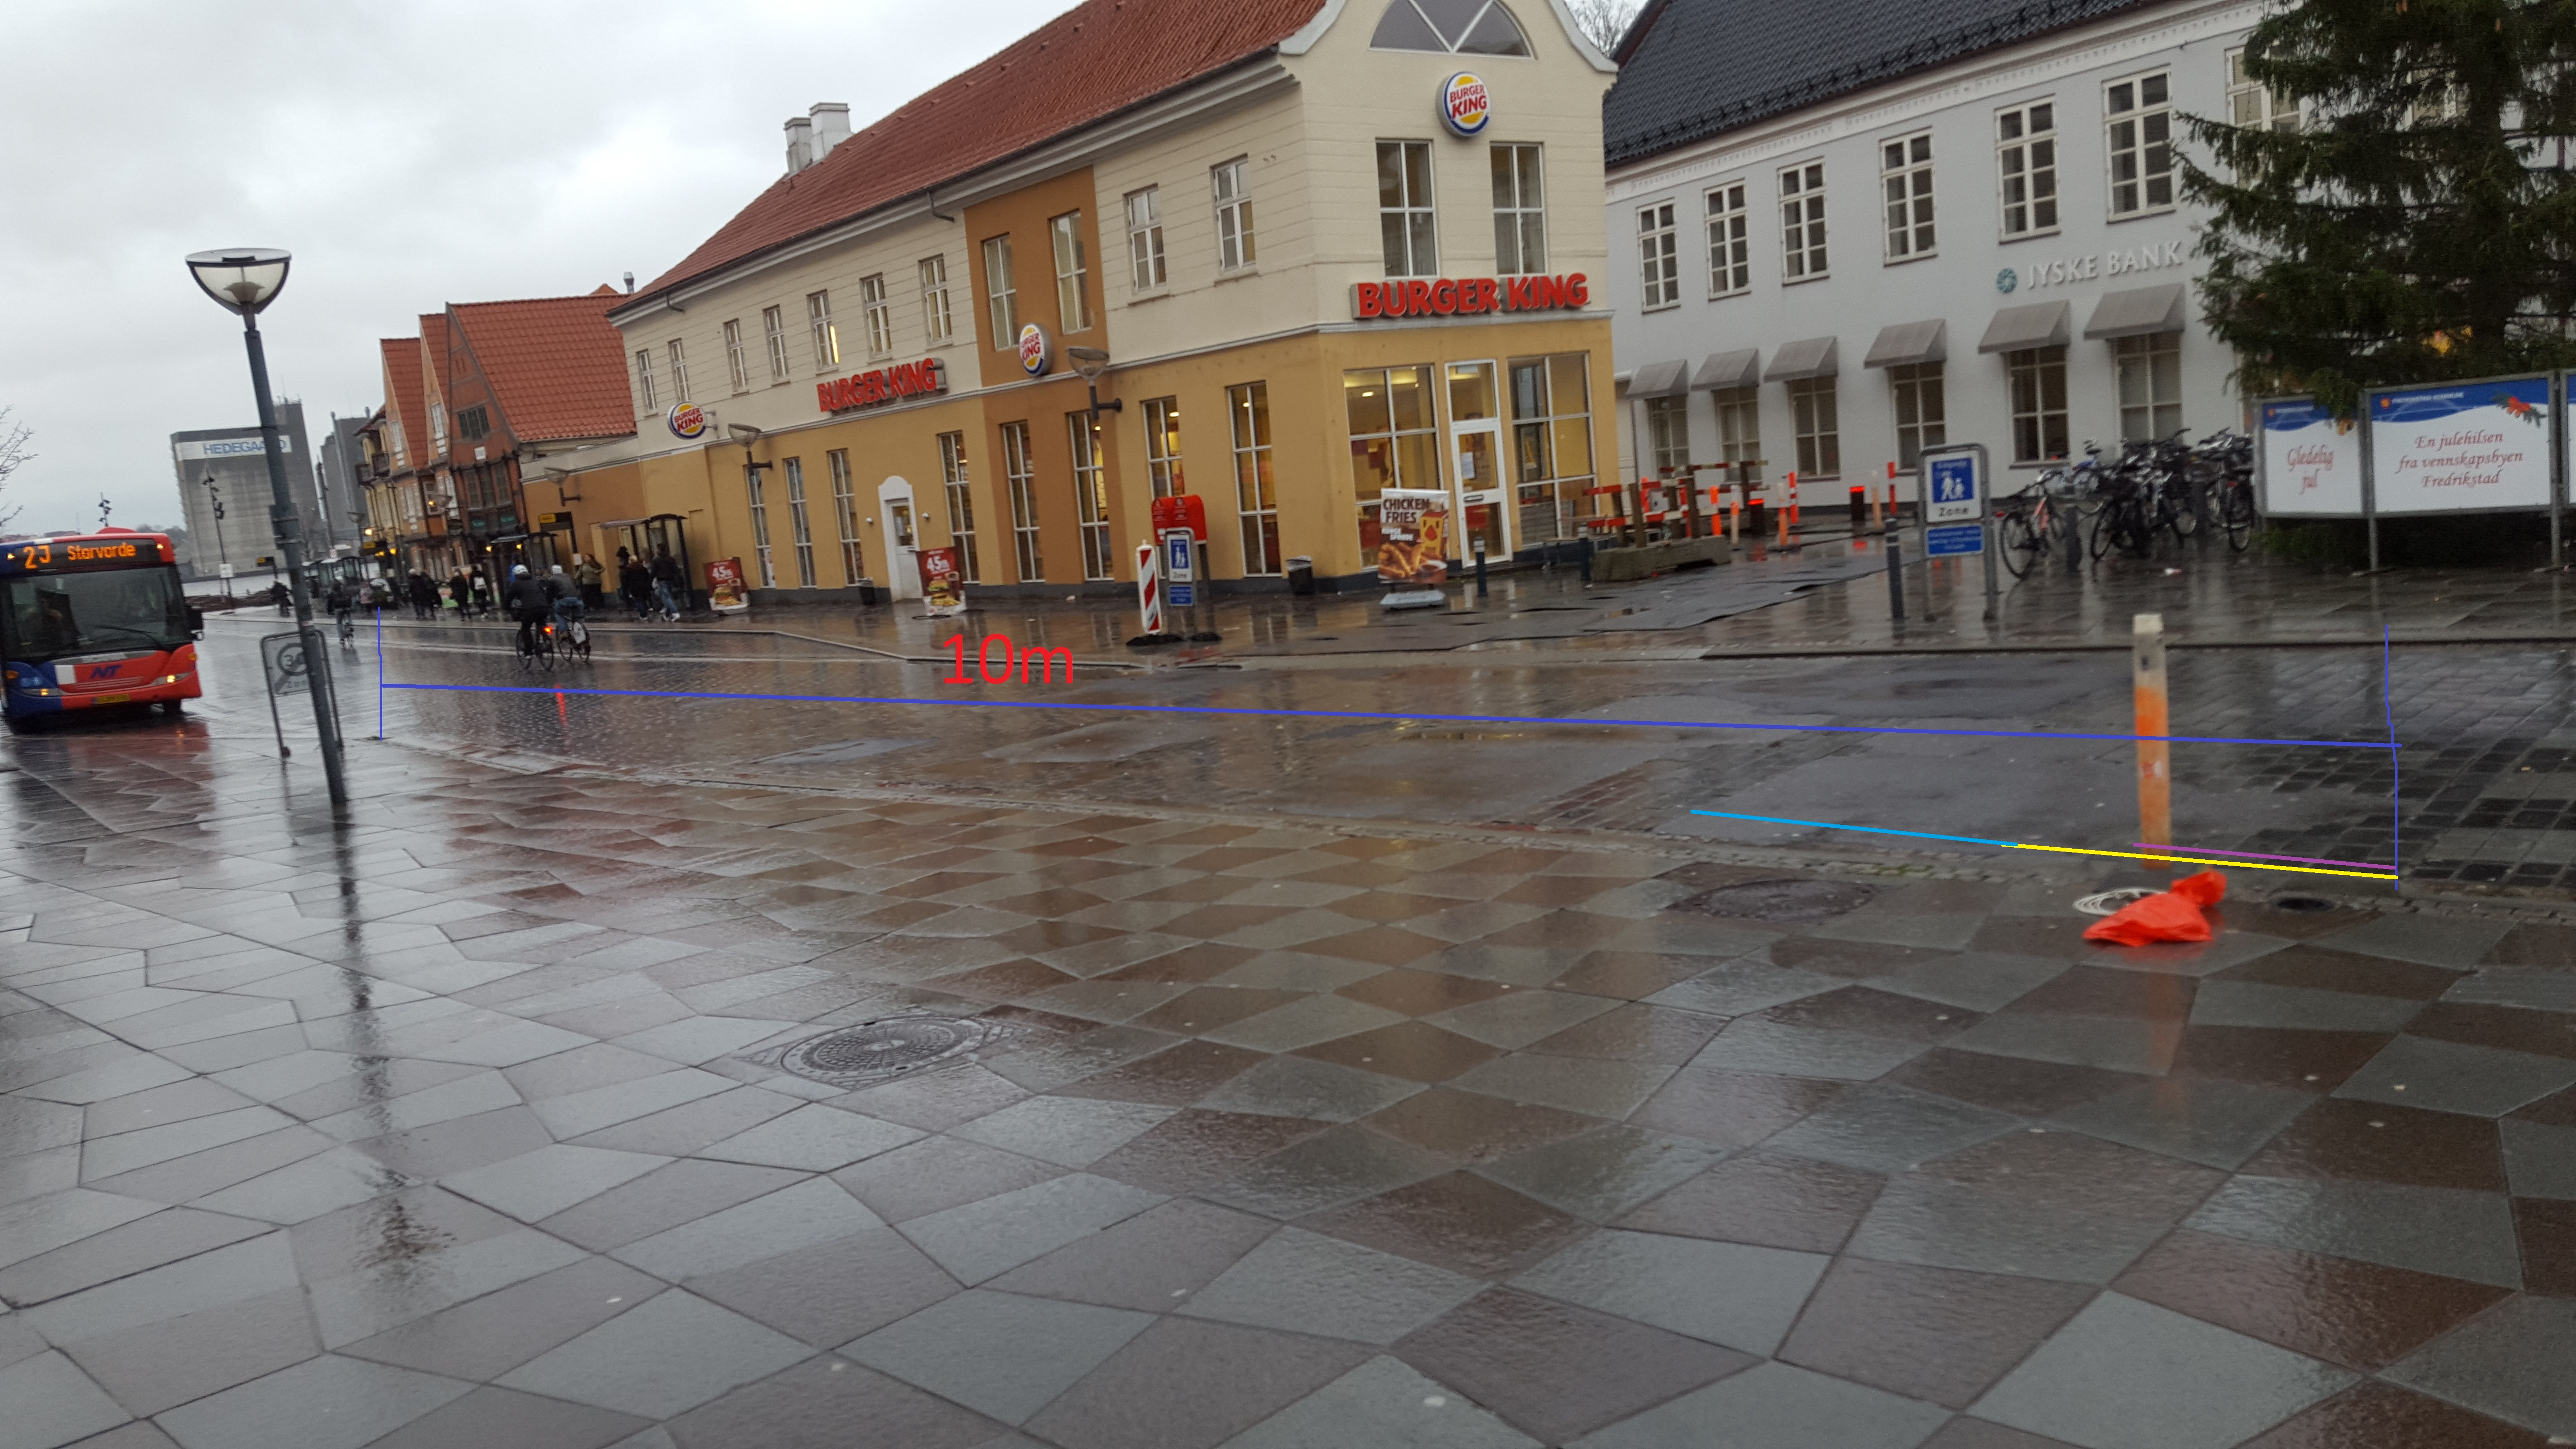
\includegraphics[width=1\linewidth]{figures/billederogfigur/blaamarkering.jpg
%	}
%	\caption{Dummy figure}
%	\label{fig:maalingerfrabegge}
%\end{figure}



%\begin{figure}
%\centering
%\begin{subfigure}{1\textwidth}
 % \centering
  %\includegraphics[width=1\linewidth]{figures/billederogfigur/rodmarkering.jpg}
  %\caption{A: Måling fra den højre kant}
  %\label{fig:obsomrrod}
%\end{subfigure}
%\begin{subfigure}{2\textwidth}
 % \centering
  %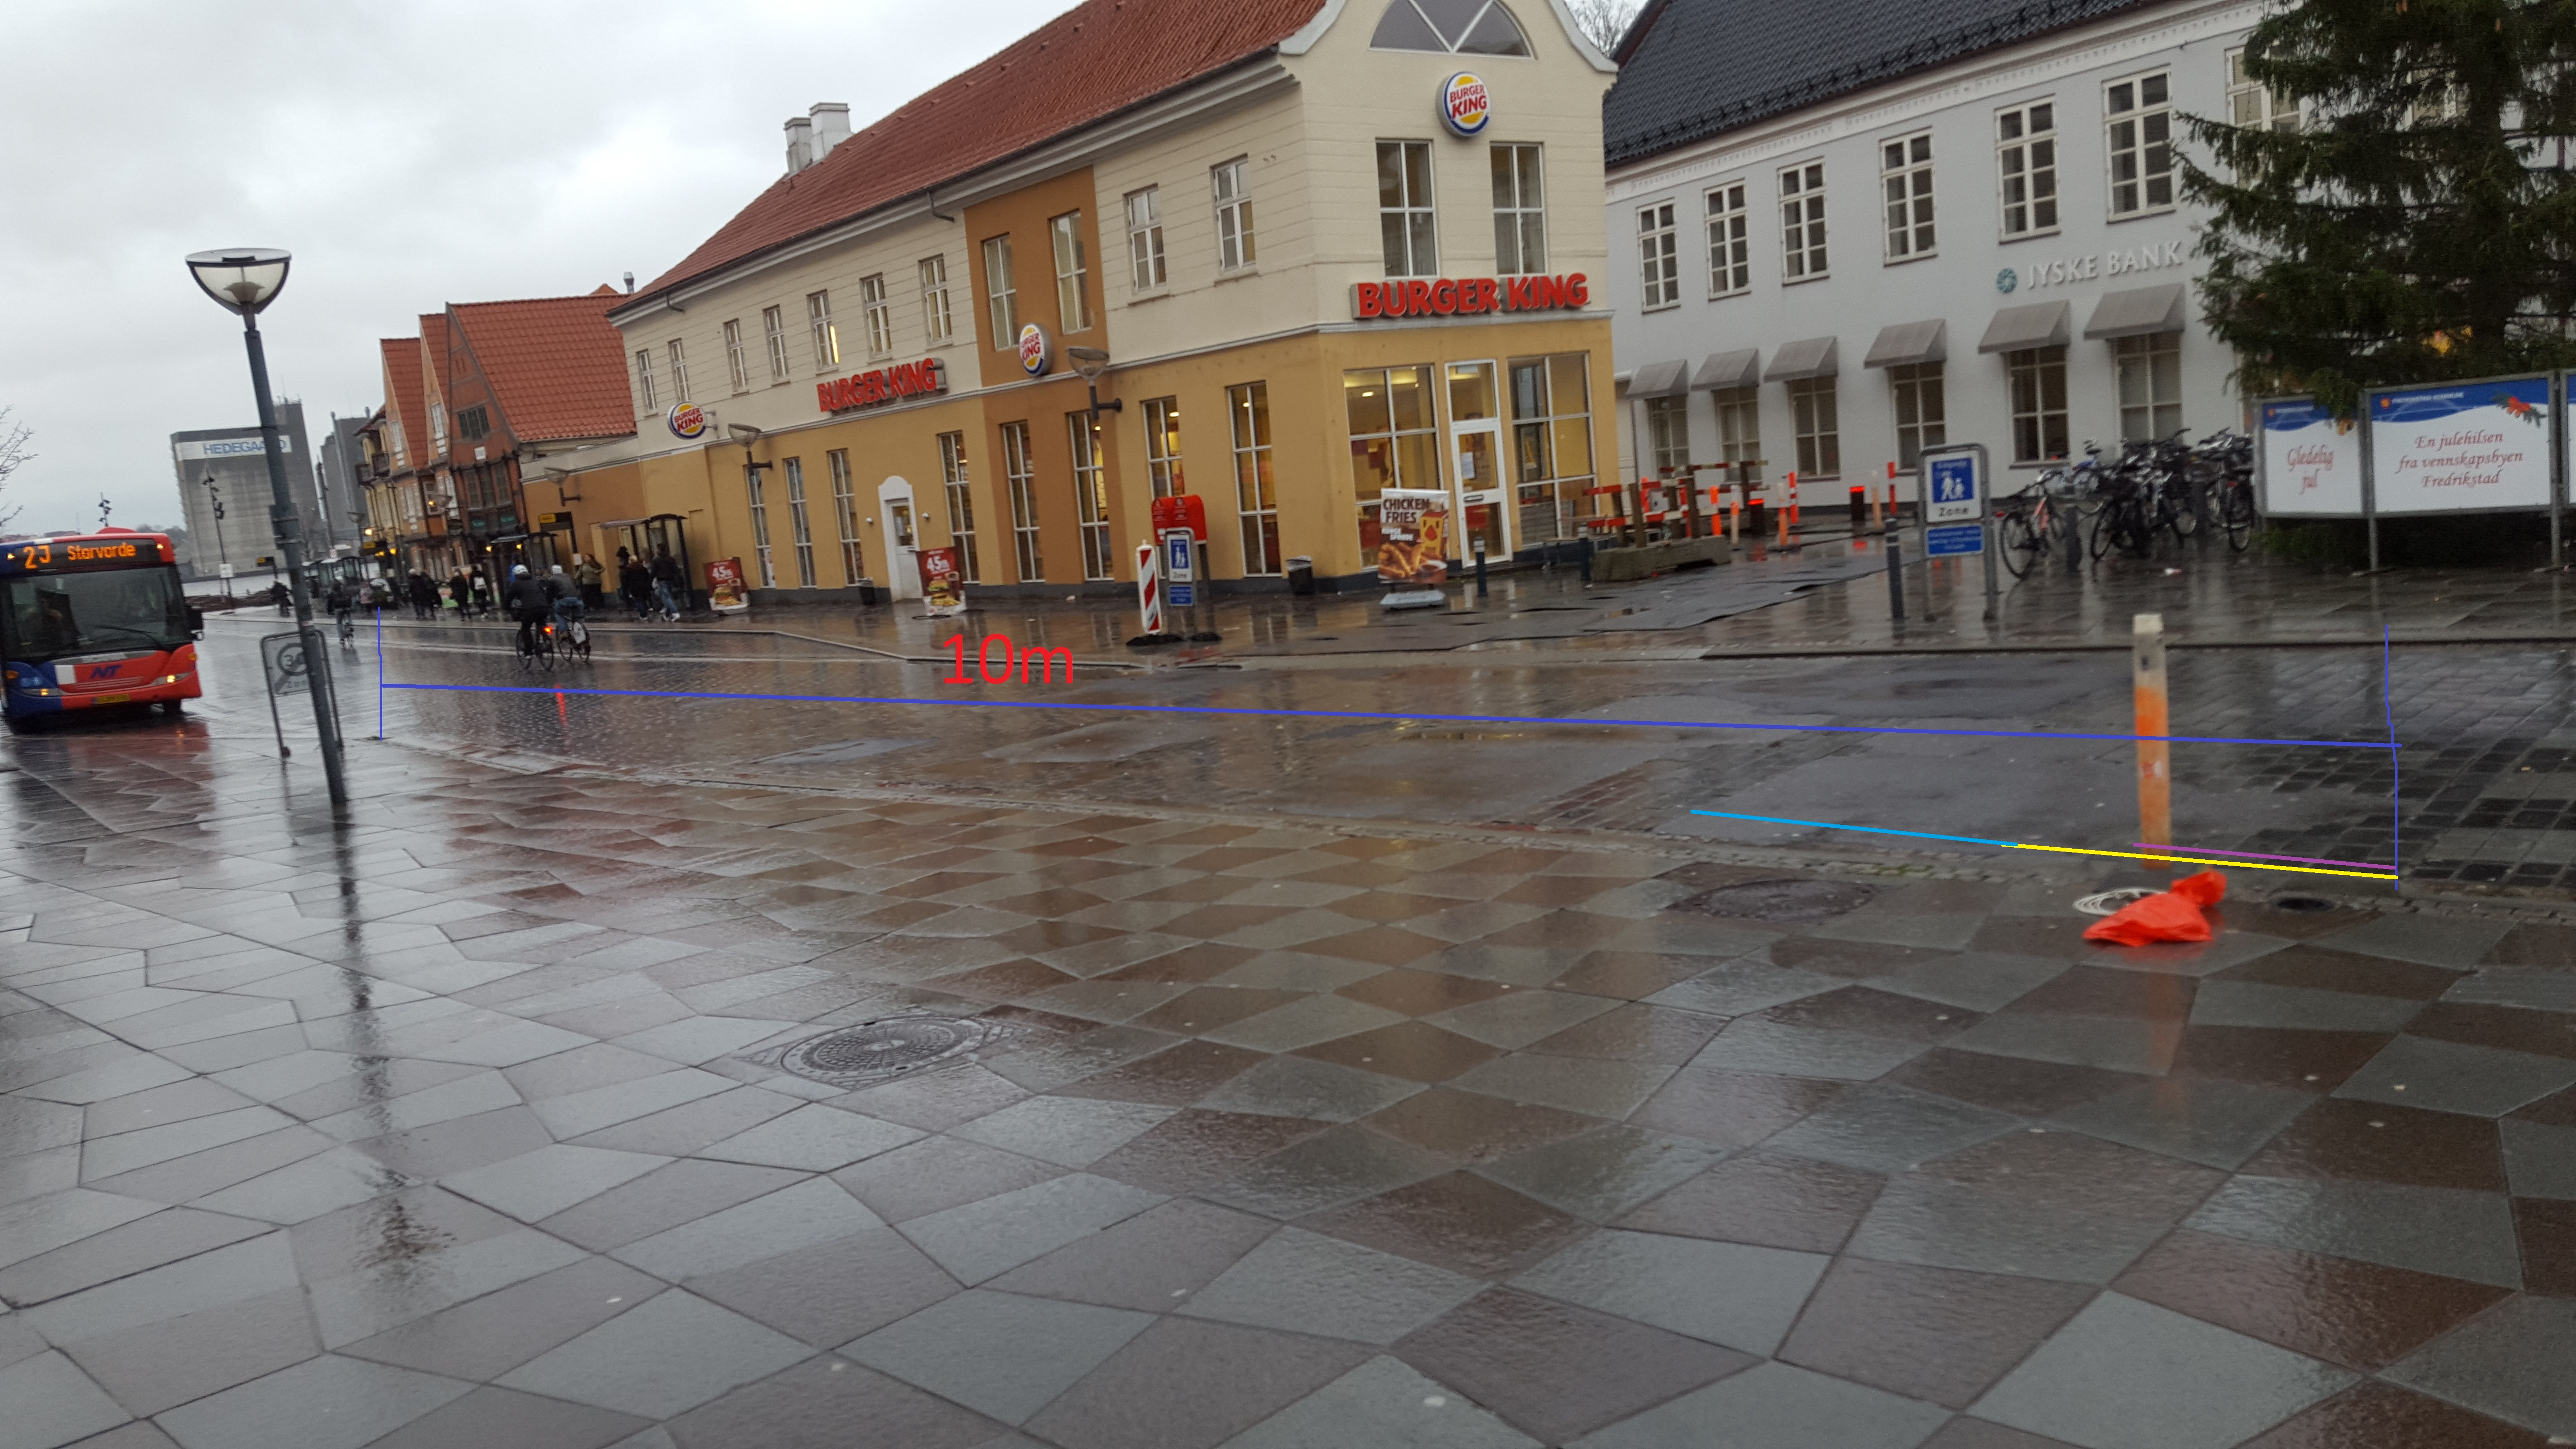
\includegraphics[width=1\linewidth]{figures/billederogfigur/blaamarkering.jpg}
  %\caption{B: Måling fra den venstre kant}
  %\label{fig:obsomrblaa}
%\end{subfigure}
%\caption{Målinger fra begge sider}
%\label{fig:maalingerfrabegge}
%\end{figure}
Herefter var metoden bag TA-værdien, at der blev lavet nogle målinger. De forskellige distancer blev noteret, og derudover blev der også taget tid til hver enkelt konflikt.%\\

Starttidspunkt: 13:00
%\\
Sluttidspunkt:15:00
%\\
Placering: Fodgængerfeltet ved Bispengade
%\\
Observationssted: Guiness Bar udenfor
%\\
Anvendt materiale: Computer og tidsfornemmelse, stopur
%\\
Fejlkilder: Regnvejrsdag, egen tidsfornemmelse
%\\
Afstand fra havn til fodgængerfelt, som blev brugt til at måle hastighed: 10m
%\\
Afstand fra Jyske bank til fodgængerfelt: 10m
%\\\\
I første omgang blev tiderne af TA-værdi antaget, som vises i tabellen %-cref{tab:antaget_tavardi}
\\\\
\begin{tabular}{ |p{1cm}|p{4cm}|p{4cm}|p{4cm}|  }
\hline
\multicolumn{4}{|c|}{Antaget TA-værdier} \\
\hline
Cykel & Hastighed [km/t] & TA-værdi [s] & Distance [m] \\
\hline
1 & 6   & 1.5 & 2 \\
2 & 10  & 0.7 & 0.5 \\
3 & 4.6 & 1.5 & 2 \\
4 & 11  & 0.4 & 1 \\
5 & 10  & 1 & 2 \\
6 & 9   & 0.1 & 0.5 \\
7 & 12  & 0.6 & 0.5 \\
8 & 10  & 0.7 & 1 \\
9 & 14  & 0.4 & 0.5 \\
10 & 8  & 1   & 2 \\
11 & 12 &0.3  &  1 \\
12 & 11 & 0.6 &   2\\
13 & 10 & 0.8 & 1\\
14 & 6  & 1   & 2\\
15 & 9  & 0.9 & 1\\
16 & 10 & 0.5 & 1\\
17 & 14 & 0.3 &0.5\\
18 & 12 & 0.6 & 0.5\\
19 & 7  & 1 & 2\\
20 & 5  & 1.5 & 2\\
\hline
%\caption{Antaget TA-værider}
%\label{tab:antaget_tavardi}
\end{tabular}



\subsection{Resultater af observation}
\label{sub:def_konflikt}
Som tidligere nævnt, så blev distancen for hvert konflikt noteret, hvilket gør det muligt, at beregne en mere præcis TA-værdi. Tabel %-cref{tab:beregnede_tavardi},
viser den beregnede TA-værdi for den bestemte hastighed samt distance, som blev målt under udførelsen af metoden.
\\
\begin{tabular}{ |p{1cm}|p{4cm}|p{4cm}|p{4cm}|  }
\hline
\multicolumn{4}{|c|}{Beregnet TA-værdier} \\
\hline
Cykel & Hastighed [m/s] & TA-værdi [s] & Distance [m] \\
\hline
1 & 1.6   & 1.25 & 2 \\
2 & 2.8 & 0.1 & 0.5 \\
3 & 1.3 & 1.5 & 2 \\
4 & 3  & 0.3 & 1 \\
5 & 2.8  & 0.7 & 2 \\
6 & 2.5   & 0.2 & 0.5 \\
7 & 3.3  & 0.1 & 0.5 \\
8 & 2.8  & 0.3 & 1 \\
9 & 3.9  & 0.1 & 0.5 \\
10 & 2.2  & 0.9   & 2 \\
11 & 3.3 & 0.3 &  1 \\
12 & 3.1 & 0.6 &   2\\
13 & 2.8 & 0.3 & 1\\
14 & 1.6  & 1.25   & 2\\
15 & 2.5  & 0.4 & 1\\
16 & 2.8 & 0.3 & 1\\
17 & 3.9 & 0.13 &0.5\\
18 & 3.3 & 0.1 & 0.5\\
19 & 1.9  & 1 & 2\\
20 & 1.4  & 1.4 & 2\\
\hline
%\caption{Beregnede TA-værider}
%\label{tab:beregnede_tavardi}
\end{tabular}
\\\\
%Som beskrevet i afsnit -cref{sub:def_konflikt}, så kan grafen for TA-værdien bruges til at identificere, hvor alvorlig konflikterne egentlig er ved området. I grafen kan der ses, hvor de beregnede TA-værdier er placeret, altså om de tilhører en alvorlig konflikt eller ej.
Som beskrevet i afsnit %-cref{sub:def_konflikt},
så kan grafen for TA-værdien bruges til at identificere, hvor alvorlig konflikterne egentlig er ved området. I grafen kan der ses, hvor de beregnede TA-værdier er placeret, altså om de tilhører en alvorlig konflikt eller ej.
%!!(GRAF skal laves, hvor der er en tildeling af konfliktgraderne, herunder skal beregnede TA-værdier sættes ind)!!
Som der kan ses på grafen, så er størstedelen af konflikterne ret alvorlige, eftersom trafikanterne kommer ret tætte på hinanden ved nogle bestemte hastigheder.
%\\\\
Mens den svenske trafikteknik blev udført ved området, blev der også udført adfærdsregistering ved området. Metoden bag adfærdsregistering vil blive introduceret inden udførselen bliver præsenteret.
Når	man	vil	observere nogle	konflikter mellem to eller flere	forskellige trafikantgrupper,	må man lave	nogle antagelser	om, hvad	 der egentlig vil føre til en konflikt. Man må altså	på	forhånd	opstille nogle hypoteser, som man via nogle undersøgelsesspørgsmål, kan bruge til	at forudse nogle	formåede	konflikter mellem nogle bestemte	trafikantgrupper.	Baggrunden for denne	måde at	undersøge konflikter	på ligger i,	at man sjældent 	vil	have	mulighed	 for at	observere selve konflikterne	eller uheldene, da det ikke	vil	være	 dagligdag på	 det	 givne observationssted.	I denne	undersøgelse om	fodgængernes tryghed på	Nytorv,	vil man altså ikke på observationsdagen formode,	at man direkte vil observere en alvorlig	 konflikt eller	et uheld mellem	en fodgænger og	en cyklist.	Måden man derimod	vil	kunne undersøge	de opstillede hypoteser på og bygge sine	spørgsmål op omkring, vil	være	at bruge en	evalueringsmetode, hvor	man	kigger på adfærdsstudier.i Her fokuserer	man	på den typiske normale adfærd på	sit observationssted, og	det skal så	underbygge	hypoteserne. Hele ideen bag denne evalueringsmetode er at ”forcere indhentningen af data”	(samme	kilde),	altså at forudsige data	som	belæg for sine antagelser.
I denne undersøgelse vil	adfærdsregistreringen blive bygget op omkring	 %-cref{fig:adfreg},
hvor fokus ligger på dels ankomsten mellem fodgængere	 og cyklister og dels ankomsten mellem	fodgængere og biler på observationsstedet. Udgangspunktet herfra er så at	undersøge, om	der i samtidige ankomster er	et tidligt samspil eller	et sent samspil mellem de to trafikanter.
Herefter vurdere, om hændelse ud fra	de to parametre gik godt, om	der	opstod en konflikt	eller der decideret skete et	uheld. Hypotesen er	så,	at hvis	antallet af	tidlige samspil stiger og antallet af sene samspil falder, så vil trafiksikkerheden, og derved trygheden, blive forøget.
\begin{figure}[htbp]
  \centering
  \begin{adjustbox}{max width=\textwidth}
    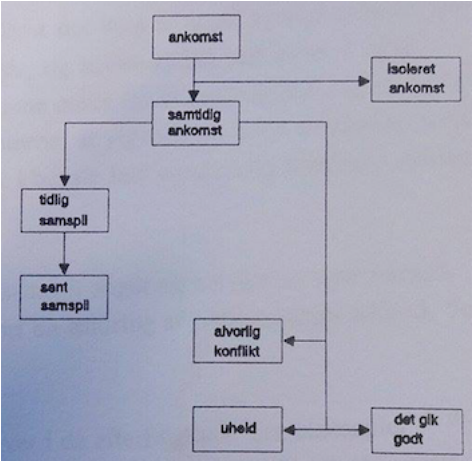
\includegraphics[scale=0.7]{figures/Billederogfigur/adfaerdsreg.png} %papir fra vejledern
 \end{adjustbox}
  \caption{Adfærdsregistrering}
    \label{fig:adfreg}
\end{figure}
%~\\\\
\subsection{Adfærdsregistrering}
\label{sub:adfregis}
Dette afsnit er udarbejdet ud fra kilden: Konfliktteknik og adfærdsstudier.
%\\
For	at kunne registrere den typiske normale adfærd ud	 fra figuren, er det vigtigt at definere	de	forskellige	begreber. I tabel (??) kan man se en	opdeling af de forskellige begreber, en definition af dem og en optælling af de forskellige tilfælde. Alle	tilfældene finder sted i	en samtidig ankomst, da der i en isoleret ankomst	 ikke vil kunne	opstå en konflikt mellem to parter. En samtidig ankomst er i vores undersøgelse defineret som cyklisten eller bilens ankomst ”til konfliktpunktet mindre end 2.5 sek efter eller mindre end 1.0 sek før fodgængeren.” (kilde udleveret	litteratur)	Ligeledes skal cyklen	eller bilen ikke være påvirket af andre parter. De skal altså være fritkørende. Definitionen på en fritkørende bil eller cyklist	vil	være, at de ikke er styret af nogle	forankørende eller tæt bagvedkørende, som eventuelt ville kunne påvirke fart og opmærksomhed.
\\\\
\begin{figure}[htbp]
  \centering
  \begin{adjustbox}{max width=\textwidth}
    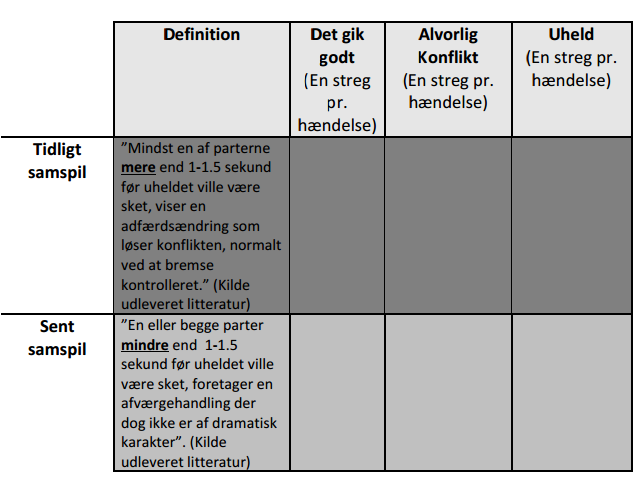
\includegraphics{figures/Billederogfigur/obstabel.png} %papir fra vejledern
 \end{adjustbox}
  \caption{Adfærdsregistreringstabel}
  \label{fig:adfregtabel}
\end{figure}
%\\\\
\textbf{"Det	gik	godt"} er defineret som en passering af konfliktpunktet, hvor situationen
har	været under kontrol og der har været afstand mellem parterne.8
%\\\\
\textbf{"Alvorlig konflikt"}	er defineret ud af en afværgehandling, som ville have ført til en kollision mellem to parter. Afværgehandlingen sker inden for 1-1.5 sekund før den mulige	kollision%(udleveret	litteratur).
%~\\\\
\textbf{"Uheld"} er defineret ved en kollision mellem to parter.
%~\\\\
Bemærk ved udførselen af denne metode blev der set bort fra isolerede ankomster, eftersom det ikke ville have haft indflydelse på vores konflikanalyse. Herefter blev målingerne fra TA-værdien brugt, hvilket kan ses på -cref{fig:maalingerfrabegge}, og alt andet ved observationen er det samme som det forrige %-cref{sub:dyb_undersoelse}
, hvor TA-værdien blev undersøgt.
%~\\\\
Det blev taget tid for hver reaktion for konflikt, således der kunne identificeres om der var sensamspil eller tidlig. Derudover blev der også set om konflikten gik godt eller om der var tale om alvorlig konflikt, som er defineret som sensamspil. De opnåede resultater kan ses på %-cref{fig:adfregtabelresult}.
Resultaterne fra TA-værdi og adfærdsregistering sættes sammen
\begin{figure}[htbp]
  \centering
  \begin{adjustbox}{max width=\textwidth}
    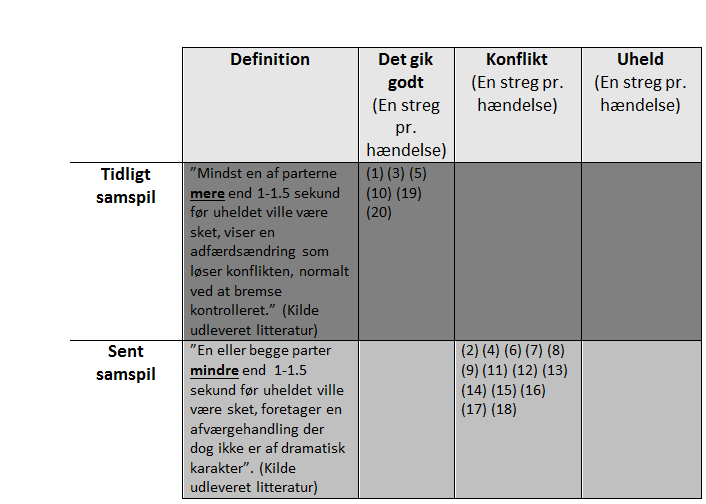
\includegraphics{figures/Billederogfigur/obstabelresult.png} %papir fra vejledern
 \end{adjustbox}
  \caption{Adfærdsregistreringstabel med resultater}
  \label{fig:adfregtabelresult}
\end{figure}
Der var en hypotese om, at hvis antallet af tidlige samspil stiger og antallet af sene samspil falder, så vil trafiksikkerheden og trygheden fra området blive forøget. Ses der på adfærdsregisteringen -cref{fig:adfregtabelresult}, så kan der observeres, at der var flere sene samspil end tidlige samspil. Det vil ifølge vores hypotese pege på, at sikkerheden samt trygheden er dårlig ved netop dette sted. Ud fra TA-værdien kunne der også bekræftes, at sikkerheden og trygheden ikke er helt optimalt.
Ud fra TA-grafen kan der ses, at 7 ud af 20 konflikter ikke er alvorlige, hvoraf 13 ud af 20 er alvorlige. Det svar til, at 65 procent af konflikterne er alvorlige, hvoraf resterne 35 procent er mindre alvorlige, og som ikke har en stor betydning for områdets sikkerhed.


\section{Løsningforslag}
Dette afsnit kommer med konstruktive løsningforslag, som har til formål, at optimere trafik flowet og øge sikkerheden. Der er arbejdet ud fra rapportens undersøgelse af trygheden i området, hvor hvert løsningforslag har sin egen individuelle indflydelse på nogle af problemerne. Det er tænkt, at alle løsningforslagene vil kunne blive indført samtidigt, og de i samspil vil kunne optimere mest muligt.

\subsection{Cykelbane som løsningforslag for et tryggere område i Nytorv}
\label{sub:Cykelbane_som_loesningforslag_for_et_tryggere_omraade_i_Nytorv}
I dette afsnit er forskellen på en cykelsti og cykelbane beskrevet, da de har hver deres udformning.  Dermed er der foretaget nogle mål og tegninger for, hvordan en ruteplanlægningen kunne se ud i Nytorv/Østerågade og gennem Boulevarden. 

\subsection{Forskellen på cykelsti og cykelbane}
\label{forskelpaacykelsti}
Både fodgænger og cyklister oplever trængsel og en vis form for utryghed i Nytorv/Østerågade området \cref{chapter:interview}. Ifølge flere interviewpersoner, som medvirkede i interviewet på Nytorv/Østerågade bliver fodgængere og forbigående cyklister utrygge, af manglende plads til cyklisterne på kørebanen i området, hvilket resultere i at cyklisterne benytter sig af fortovet \cref{chapter:interview}. Derfor vil det være praktisk med nogle cykelstier eller cykelbaner i Nytorv/Østerågade området.  
\\
Forskellen på cykelstier og cykelbaner er, at cykelstier karakteriseres ved, at de er adskilte fra kørebanen med en kantsten eller en rabat, hvor de er markeret med et rundt påbudsskilt eller med et cykelsymbol på stien. \autocite{vejdpdf}Cykelbanen er udformet som vist i figur.  


%BILLEDET OM CYKELSTIEN MANGLER

 \begin{figure}[htbp]
   \centering
   \begin{adjustbox}{max width=\textwidth}
     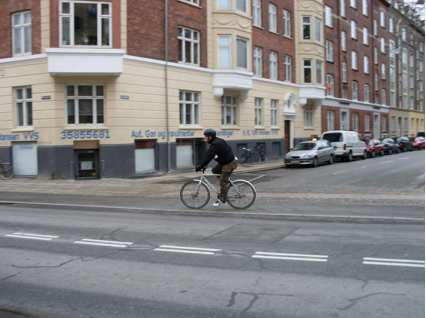
\includegraphics{figures/Billederogfigur/cykelsti.png}
  \end{adjustbox}
   \caption{Cykelsti}
    \label{fig:cykelsti}
 \end{figure}

En cykelbane er en bane, som deler vejen med kørebanen. Den er kun afgrænset mod kørebanen med 30 cm bred udbrudt kantlinje. Heraf har cykelbanen status som en cykelsti, og er ofte markeret med et rundt påbudsskilt eller med et cykelsymbol på vejen. En cykelbane etableres, hvis der kun er få cyklister, langsomt kørende biler, ved økonomiske eller pladsmæssige årsager \autocite{vejdpdf}.   Ifølge bekendtgørelsen om anvendelse af afmærkninger, kan almindelige vognbaner adskille sig fra blandt andet cykelbaner, hvor kantlinjen skal udføres bred \autocite{lovb}.  

\subsection{Cykelbane i Nytorv/Østerågade}
En cykelbane i Nytorv/Østerågade kan en cykelbane ifølge interviewpersonerne bl.a. udløse mere tryghed i området (se bilag), da der på nuværende tidspunkt er manglende vejplads til cyklisterne. Herved kunne den generelle cykelsti udformes som følgende ruteplan. Målene og billedet er taget fra kilden ... fra http://iform.dk/ruteplanner/tegns .

RUTEPLAN BILLEDE
 \begin{figure}[htbp]
   \centering
   \begin{adjustbox}{max width=\textwidth}
     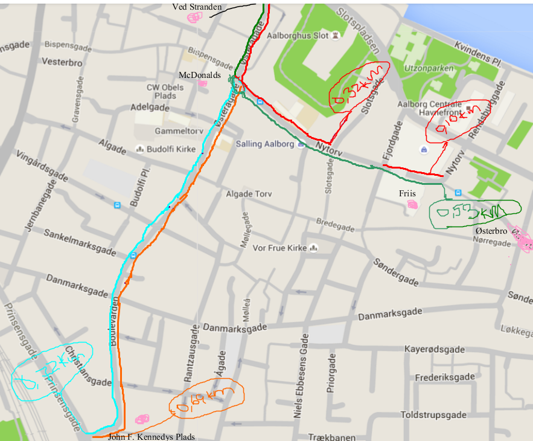
\includegraphics{figures/Billederogfigur/ruteplanlaegning.png}
  \end{adjustbox}
   \caption{Ruteplanlægning}
    \label{fig:ruteplan}
 \end{figure}
Cykelbanen kunne laves fra enden af Friis til Ved Stranden på højre og venstre side, rundt om pladsen foran McDonalds, også videre mod Østerågade. Følgende billeder er taget fra https://www.google.com/maps. 

3 BILLEDER MANGLER
\begin{figure}[htbp]
  \centering
  \begin{adjustbox}{max width=\textwidth}
    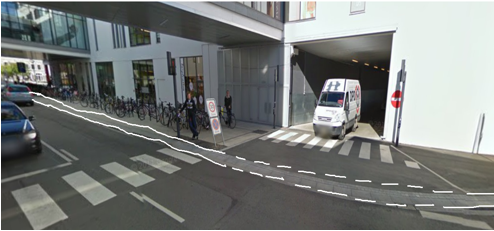
\includegraphics{figures/Billederogfigur/friiscykeltsti.png}
 \end{adjustbox}
  \caption{Cykelsti ved Friis}
   \label{fig:cykelsti_friis}
\end{figure}

\begin{figure}[htbp]
  \centering
  \begin{adjustbox}{max width=\textwidth}
    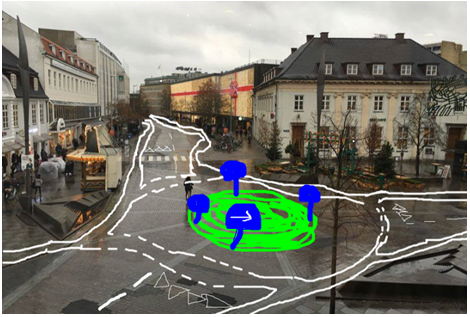
\includegraphics{figures/Billederogfigur/cykelsti_ved_mac.png}
 \end{adjustbox}
  \caption{Cykelsti ved MacDonald}
   \label{fig:cykelsti_mac}
\end{figure}
\begin{figure}[htbp]
  \centering
  \begin{adjustbox}{max width=\textwidth}
    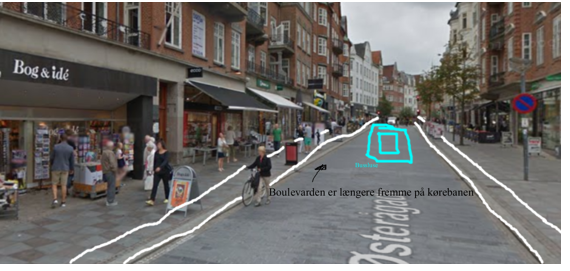
\includegraphics{figures/Billederogfigur/bogogide.png}
 \end{adjustbox}
  \caption{Cykelsti mod Boulevarden}
   \label{fig:cykelsti_boulevarden}
\end{figure}





Ved Østerbro er der blevet lavet en cykelbane midt på fortovet, på samme måde kunne en cykelbane i de ovenstående områder laves. 

CYKELSTI VED ØSTERBRO
\begin{figure}[htbp]
  \centering
  \begin{adjustbox}{max width=\textwidth}
    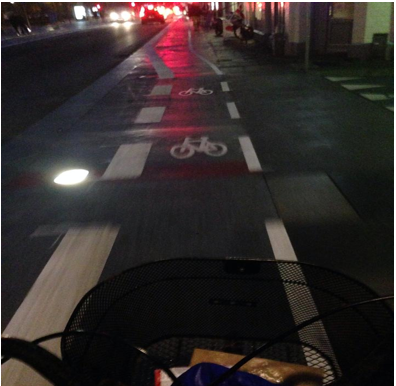
\includegraphics{figures/Billederogfigur/osterbro.png}
 \end{adjustbox}
  \caption{Cykelsti ved Østerbro}
   \label{fig:cykelsti_ved_osterbro}
\end{figure}


\subsection{Vurdering af løsning på problemet i Nytorv/Østerågade}
Fordelen ved at etablere en cykelsti eller cykelbane er, at hver trafikantgruppe vil føle sig mere trygge af at de var delt. Ifølge en interviewperson bliver folk utrygge af, at \emph{”(…) fodgængere, cyklister og biler nærmest deler vejen, og at det ikke alle der tager hensyn til hinanden, vil føle mig mere tryg hvis vi var delt.”} En differentiering mellem trafikantgrupperne vil virke mere betryggende, end hvis de forskellige trafikantgrupper skulle dele vejen, her af vil det være en fordel at få etableret en cykelbane med kantlinjer frem for en cykelsti med en kantsten eller en rabat, da den kræver plads, at få udført en cykelbane. Ulempen ved at have en cykelbane er at der cykler mange ud imod området, det mener en interviewperson, at \emph{“(…)om morgenen så er der fart på her i området, altså mange folk cykler mod skoler, universitet og på arbejde(…)”}. Det vil i vissetilfælde resultere i, at cykelbanen bliver proppet og at cyklisterne vil fordele sig på kørebanen og længere ud på fortovet. I den forstand vil cykelbanen ikke afvikle morgentrafikken godt nok. Heraf kunne en cykelbro være mere praktisk men dog vil den være dyr at finansiere.  Derudover er der risiko for, at fodgængere ikke vil benytte sig af cyklisten, hvilket kan skabe et sammenstød mellem fodgængere og cyklister.  
\\

BILLEDER, KILDEHENVISNING OG GENERELLE RETTELSER MANGLER

%\subsection{Hvidt fodgængeroverfelt}
\label{sub:hvid_fordgaengeroverfelt}

\subsection{Rundkørsel}
\label{sub:rundkoersel}
En løsningsforslag kan være rundkørsel. Ved blot at kigge på rundkørsel, så kan der hurtig ses, at farten vil blive sænket ved de områder hvor der er rundkørsel. Får man indført rundkørsel ved Nytorv området, så vil hypotesen være at cyklister pr. automatik sænker farten ved området, hvilket øger TA-værdien ved området.  Ifølge artiklen “Rundkørsler og trafiksikkerhed” så bliver beskrevet, at rundkørsler vil optimere sikkerheden for fodgængere, hvilket er en af de problemer ved Nytorv området. Ifølge kilden så formindskes cykel sikkerheden ved, at der biler som også skal bruge rundkørslen. Men dog så er biler ikke tilladt, at køre ved Nytorv området, men idet at der alligevel passere personbiler, så er de meget forsigtige. Så ergo kan der antages, at rundkørsel kan være med til, at optimere sikkerheden for cyklister. I tilfælde man skal opbygge en rundkørsel i området, så vil placeringen være, som der ses på billedet:

 \begin{figure}[htbp]
   \centering
   \begin{adjustbox}{max width=\textwidth}
     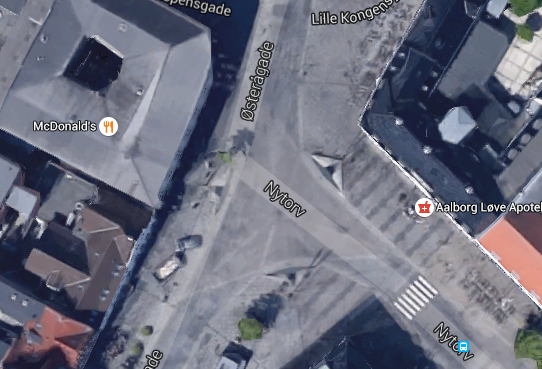
\includegraphics{figures/Billederogfigur/rundkorselplace.png} %googlemaps
  \end{adjustbox}
   \caption{Placering af Rundkørsel}
    \label{fig:rundkorselplace}
 \end{figure}
 \newpage

%rundkorselplace.png
\subsubsection{Fordel og Ulempe}
\label{subs:fordel_og_ulempe}
En fordel ved rundkørsel ved Nytorv området vil være, at alle trafikanter kan færdes uden fare for konflikter, eftersom farten vil bliver sænket drastisk forhold til hvad den er allerede. Derudover vil der blive skabt mere tryghed og sikkerhed for fodgængere, da farten ved området bliver sænket. Eftersom rundkørsel har sine fordele, så har den lige så vel ulemper. Den største ulempe vil nok være, at der mange busser der færdes ved området og skarpe sving er dog ikke det optimale for busser, så det vil skabe forsinkelser i og med, at flere trafikanter skal færdes i et område. En anden ulempe er nok, det kan blive farligt for cyklister, da der er personbiler som krydser Nytorv illegal og ifølge artiklen “Rundkørsler og trafiksikkerhed”, så vil personbiler blive farligt for cyklister ved en rundkørsel.

\subsubsection{Løsning eller ej?}
\label{subs:Losning}

Som umiddelbart vil rundkørsel lyde til, at være en fantastisk ide, eftersom det kan sænke alle mulige uheld med 47 procent. Der kan så antages, at det nok også vil sænke faren for alvorlige konflikter ved området Nytorv. Ifølge observationen, så var der 13 ud af 20 konflikter som var alvorlige, hvis dette kan sænkes med 47 procent, så vil det svar til ca. 6 ud af 20 konflikter vil blive mindre alvorlig. Dog har løsningsforslaget sine ulemper, som kan gøre Nytorv et meget stresset sted for alle trafikantgrupper. Derudover vil det også gå ud over butikker der er  ved området eftersom der kan opstå nogle lange køer ved området.

\subsection{Bussluse som løsningforslag for et tryggere område i Nytorv/Østerågade}
\label{bussluse som løsningforslag for et tryggere område i Nytorv/Østerågade}

I dette afsnit er forskellen på bus sluserne beskrevet, da de har forskellig udformning. Der overvejes et løsningforslag, som kan bruges i området på Nytorv/Østerågade. Forslaget vil udmunde beskrivelse og tegninger for, hvordan en løsning kan se ud på Nytorv/Østerågade og gennem Boulevarden.      
\\\\
I Aalborg har man tidligere anvendt bus sluser på mange steder, som ved skoler og områder med stilleveje. På Nytorv/Østerågade ligger mange restauranter, shoppingfaciliteter og cafeér, og som nævnt tidligere, er der mange mennesker, som færdes i området. Samtidig er der forbud af gennemkørsel af privatbiler i området, men det er aldrig blevet respekteret fuldt ud, da mere end 3000 biler passerer Østerågade hver dag. (3000 biler passerer hverdag Østerågade som står i P1 projektkatalog under Nytorv/Østerågade - Problemstilling)
\\\\
Busgrav og hæve sænke pullerter er forskellige måder at lave bus sluser på.
En busgrav er ofte et hul eller en forhøjning i midten af vejbanen. I busgrave er bredden på hullet tilpasset bredden på bussens hjulpar. Dvs. at kun busser kan passere slusen, hvorimod privatbiler, med mindre bredde mellem hjulparene, vil falde i hullet. På hver side af hullet, er der ofte forhøjninger så privatbiler går i stykker, hvis de prøver at kører højre eller venstre om slusen. 
\\\\
Hæve sænke pullerter består af flere cylindre -pneumatik med en bestemt afstand mellem hver cylinder. Standart størrelsen som f. eks. 250 x 500 mm (diameter gange højde) eller 200 x 500 mm osv. Produktet kan styres ved hjælp af tidsstyring og/eller fjernbetjening ( http://www.g9-se.se/regulering-i-byrum.html ). Når en bus nærmer sig mod cylinderne, så sænkes cylinderne pr. automatik. 

             


          Byrum’s automatisk hæve sænke. Bilder fra %http://www.g9.dk/media/blfa_files/Luxor_pullert.pdf


\subsection{Bussluserne i Nytorv/Østerågade}
\label{bussluse i Nytorv/Østerågade}                                           
                                           
                                           
                                         Fotograf af Rong’s mobil, og udarbejder Rong Liu
Hæve sænke pullerter som cylinder -pneumatik udføres som følgende. Ved Stranden med retning mod Østerågade kan laves cylinder -pneumatik. Privatbilister kan svinge før bus slusen og finde parkering til deres biler, og gå på Østerågade området. 
                                        
                                        
                                        
                                         Fotograf af Rong’s mobil, og udarbejder Rong Liu
Under Aalborg biblioteket er der skilte med indkørsel forbudt for privatbiler, men de kører alligevel igennem. Her kan der ligeledes placeres cylinder - pneumatik under biblioteket. Dermed undgår at privatbiler kører denne vej. Privatbiler kan parkere i Friis’s parkeringshus, i Føtex eller hos Salling.                         
                                                   
                                                   
                                                   
                                        Fotograf af Rong’s mobil, og udarbejder Rong Liu

På Boulvarden kan der placeres cylinder - pneumatik. På dette sted er der ligeledes indkørsel forbudt for privatbiler, men ikke alle overholder denne skiltning. Privatbiler kan svinge før korsvej på Vingårdsgade og parkeringer deres biler ved Budolfi Kirke eller på Budolfi Plads. 
                                                
                                                
                                       Fotograf af Rong’s mobil, og udarbejder Rong Liu
Disse løsninger er et forsøg på at gøre Nytorv/Østerågade delvist privatbilfrit. Der er derfor kun tilladt for busser og cyklister. Det må og vil give mere sikkerhed til fodgængere.

Bus sluser som hæve sænke pullerter er mere praktisk og vil forhindre gennemkørsel af privatbiler, således kun busser kan køre igennem. Hermed undgås privatbilstrafik inde i området. Hæve sænke pullerter vil aldrig skade biler, ligesom bus grave vil gøre, og fodgængere og cyklister vil heller ikke falde i “hullet”. Det vil give et tryggere område for cyklisterne og fodgængerne. 


\chapter{Diskussion}
\label{chap:diskussion}
For at kunne afgøre hvad eller hvilke eventuelle løsningsforslag, som løser rapportens undersøgte problemer bedst, er det væsentligt at se på fordele og ulemper ved de forskellige forslag. Ved at etablere en rundkørsel skabes, vil alle trafikantgrupper blive tvunget til at øge deres trafikale fokus, som konsekvens af rundkørslen. Samtidig må det forventes, at deres hastigheder må blive sænket en del. En af ulemperne ved at anlægge en rundkørsel vil på sigt blive en ringere offentlig transport i området, da det kan forsinke bustrafikken at føre dem gennem en rundkørsel på en trafikeret dag. En rundkørsel er særdeles effektiv at bruge som løsningsforslag et sted, hvor der er mange biler, som skal gennem et punkt. Eftersom det største problemfokus på Nytorv ikke er bilerne, men derimod cyklisterne, vil en rundkørsel muligvis gøre mere skade end gavn, hvis en sådan etablering blev en realitet.
Hvis der i stedet rettes fokus på løsningsforslaget med at anlægge en busgrav eller hæve-sænke pullert, er dette forslag, som det forrige, også fokuseret på bil problemet omkring Nytorv. Det ville afhjælpe problemet med de mange uvedkommende biler, der hver eneste dag kører ind i området, trods påbud, som tilsyneladende ikke har den ønskede virkning. En af fordelene bliver hermed, at Nytorv bliver helt fri for uvedkommende biler, og dette vil medvirkende til at skabe et mere forudsigeligt og måske mere trygt trafikmiljø.
Det sidste løsningsforslag beskæftiger sig med en anlægning af cykelbaner i hele området og omkring Nytorv. Fordelene er, at dette er med til at øge fokus på cyklisterne, og det giver et mere klart billede af, hvor cyklerne skal være på vejen. En af de overvejende ulemper er, at en cykelbane vil skabe gnidninger mellem cyklisterne og buspassagererne, når de skal af og på bussen. En cykelbane vil nemlig være etableret langs buslommen, og derved vil buspassagerende være nødsaget til at gå over cykelbanen. Det vil derfor være en nødvendighed, at cyklisterne er opmærksomme og holder tilbage for passagerende.
Da der i forvejen er et forholdsvis smalt fortov nogle steder nede ved Nytorv, bliver det ligeså svært at få plads til de eventuelle cykelbaner. De to første løsningsforslag har fokus på eventuelle bilproblemer, hvorimod det sidste løsningsforslag har til formål at afhjælpe cykelproblemer i trafikken. Eftersom det største trafikale problem nede ved Nytorv er mellem cyklister og fodgængere, er det oplagt at videreudvikle på ideen omkring en cykelbane.
I rapporten har den helt centrale problemstilling været, at undersøge trafikale problemer mellem fodgængere og cyklister ved fodgængerfeltet. Gennem de beregnede TA-værdier og de mange interviews, er der blevet vurderet, at der er et trafikalt problem netop på dette sted mellem cyklisterne og fodgængerne. Bilerne og busserne er gennem de foretagede interviews ikke blevet vurderet til at være et stort problem, og derfor er løsningsforslaget om cykelbanen valgt at blive diskuteret her, som den bedste løsning, for netop denne undersøgelse.
En etablering af en cykelbane vil have til formål at lede cyklisten inde for en afmærket sti, og på den måde fastholde cyklisten inden for afmærkningen Der vil herved blive formået at kontrollere cyklisternes kørebane og opretholde cyklistens fokus i selve kørebanen. Det formodes, at cyklisten vil få øje på en fodgængeren hurtigere, da der ikke er andre trafikanter cyklisten nu skal holde øje med. Det kan muligvis være med til, at man vil kunne observere mange flere tidlige samspil end sene samspil ved fodgængeroverfeltet.. Et sådant formål, ville en etablering af en rundkørsel eller bussluse ikke opfylde. Set i et andet perspektiv, så kan det måske føre til flere kollisioner mellem fodgængere og cyklister, hvis cyklisten ser cykelbanen som sin helt egen bane. Der vil derfor være et dilemma, hvis der ikke bliver taget hensyn til de eventuelle passerende fodgængere eller biler, som svinger ind over cykelbanen. Derfor vil en cykelbane ikke være en endegyldig løsning på konflikterne ved fodgængerfeltet, da det kan tænkes, at der rent faktisk vil kunne opstå flere uheld end før. Men det er klart, at en cykelbane vil kunne guide cyklisterne, og have et bidrag til et mere trygt trafikmiljø på Nytorv/Østerågade området. Dog kan det diskuteres, om det er cyklisten eller fodgængeren, som vil føle sig mere tryg.

\printbibliography[heading=bibintoc]
\label{bib:mybiblio}
\appendix
\appendix
\label{appendix_start}
\chapter{Interviews}
  \label{chap:interviews}
Interview resultater med forbigående fodgængere og cyklister ved Nytorv/Østerågade i Aalborg I dette afsnit er 4 spørgsmål beskrevet, som blev stillet og svarerende fra 20 forbigående fodgængere og cykelister ved Nytorv/Østerågade, hvor de væsentlige svar er med i rapporten.

  Spørgsmål 1.
  Føler du dig tryg ved, at gå over fodgængerfeltet, når der er mange cyklister ude ved Nytorv/Østerågade i Aalborg?
\\\\
  Svar 1.
  ”Jeg føler mig tryg af, at gå over fodgængerfeltet, når der er mange cyklister. Jeg synes at de fleste holder pænt tilbage”.
\\\\
  ”Jeg er Københavner, og jeg synes, at det er mere betryggende, at gå ude på strøget i København, der cykler ingen forbi, der er kun tværgående trafik. Jeg synes, at det er værre med bilerne, også må cyklisterne gerne være herude synes jeg.”
\\\\
  ”Jeg bruger normalt lidt tid på, at se efter om cyklisterne har set mig eller om jeg selv skal stå tilbage, også går jeg over”
\\\\
  ” Jeg synes godt, at der kan være kaos herude nogle gange, og det er både cyklister, biler og busser der skaber den kaos.”
\\\\
  ”Jeg føler mig tryg, da jeg tror at cyklisterne tænker, at jeg er gammel og de skal passe lidt på, men jeg træder aldrig ud uden at se mig for, jeg passer virkelig på.”
\\\\
  “Nej - holder øje til højre og venstre, og så kommer der nogle gange også en bil som ikke skal køre herinde.”
\\\\
  “Jeg føler mig tryg og cyklerne holder tilbage for en.”
\\\\
  “Nej - cyklerne holder ikke færdselsloven og holder ikke tilbage for fodgængerne.”
\\\\
  “Jeg føler mig tryg, når jeg går over vejen. En gang imellem ser man, at nogle stopper op og andre gør ikke, men jeg har ikke noget problem med det.”
\\\\
  “Ja det er jeg - de er gode til at holde tilbage.”
\\\\
  “Egentlig ikke - jeg synes, at cyklerne kommer meget uventet og meget hurtigt. Jeg holder utroligt meget øje.”
\\\\
  “Nej egentlig ikke - de holder ikke tilbage - det er cyklerne- jeg er mere tryg ved bilerne.”
\\\\
  “Ja det gør jeg faktisk - der er mange mennesker, men jeg synes ikke det er et problem.”
\\\\
  “Ikke altid - jeg er lige hoppet over for en cyklist.”
\\\\
  ”Jeg bor lige herude. Man kan ikke gå og regne med at der ikke er andre end en selv herude, men jeg synes ikke engang at der er ret trafikeret, det kunne have været meget værre. Jeg synes at det er helt fint herude.”
\\\\
  “Cyklisterne kører sgu som en brækket arm, Så nej jeg føler mig ikke tryg.”
\\\\
  Spørgsmål 2.
  Hvad er det, der gør dig utryg/tryg, når du går over fodgængerfeltet? og hvad er det vigtigste for dig, for at du føler dig tryg i et integreret trafikmiljø?
  \\
   Svar 2.
  “Noget mere overvågning, så biler der ikke skal køre derinde, ikke kan komme ind.”
\\\\
  ”at vi fodgængere, cyklister og biler nærmest deler vejen, og at det ikke alle der tager hensyn til hinanden, vil føle mig mere tryg hvis vi var delt.”
\\\\
  “Her på Boulevarden lagde jeg mærke til at cyklisterne ikke kunne være der, så de måtte trække deres cykler på fortovet. De kunne slet ikke være der overhovedet.  Derfor stiller jeg min cykel i Arkaden og går hernede.”
\\\\
  “Jeg benytter mig af fodgængerovergangen, og det gør mig tryg.”
\\\\
  “At færdselsloven bliver overholdt.”
\\\\
  “Det må være det, men om morgenen så er der fart på her i området, altså mange folk cykler mod skoler, universitet og på arbejde. Men så længe at vi alle opmærksomme og buschaufførerne ved godt, at der er fodgængere her, så de er også opmærksomme, at området er gågade.”
\\\\
  “At folk viser hensyn til hinanden.”
\\\\
  “Folk holder automatisk tilbage - det gør de jo ikke.”
\\\\
  “At fodgængerfeltet er helligt og folk holder tilbage.”
\\\\
  “Det er at busserne og bilerne holder tilbage. Det er dem der kan lave noget skade. Jeg har gået herinde rigtig meget, og jeg har aldrig set en ulykke.”
\\\\
  “At jeg kan gå over, når jeg synes der er fri bane.”
\\\\
  “Man ved aldrig om cyklerne holder tilbage.”
  Spørgsmål 3
  Har du nogle ønsker eller forslag til, hvordan man kan binde gågaden sammen?
\\
  Svar 3
  ”Man kan ikke se fodgængerfeltet, det er ikke tydeligt nok i den grå farve. Jeg synes godt, at man kan male fodgængerfeltet hvidt.”
\\\\
  “Jeg synes bilerne skal fjernes herfra, men busserne er okay.”
  ”Jeg synes godt, at man kan lave en bilfrizone herude, og lave flere cykelstier, med nogle gennemveje.”
\\\\

  ”man kunne evt. lave en undergang eller overgang.”
\\\\
  “Det er bare fjerne alt trafikken herinde på Nytorv. Det er ganske enkelt.”
\\\\
  ”Man kunne evt. dele os mere op, så bilerne havde deres egen kørebane og cyklisterne havde en cykelsti, de kunne cykle på.”
\\\\
  “Jeg ved ikke om det er praktisk, men man kunne jo bygge en gangbro, i stedet for de fodgængere felt, men hvis man ser på højden af busserne, så ved jeg ikke om det er realistisk. Ellers så vil mit bud være, at lave en tunnel, som man har ved Aalborg banegård.”
\\
Spørgsmål 4.
Hvad synes du om, at lave en cykelsti uden om Nytorv og derved udelukke cyklisterne helt fra området?
<<<<<<< HEAD
\\\\
  Svar 4.
  ”jeg synes ikke, at man skal udelukke cyklisterne fra Nytorv, jeg synes mere at man skal udelukke privatkørsel på en eller anden måde.”
\\\\
  “Jeg ved, at butikkerne er imod, at man lukker for trafikken her i Nytorv, da de mener at deres salg vil gå ned. Men det passer altså ikke, fordi der er et gammelt universitets undersøgelse der har vist, fluger tror jeg, at det faktisk vil gå bedre hvis der kun er gågade. De vil sælge mere.”
\\\\
  ”Jeg kommer oprindeligt fra Kina, og der synes jeg ikke at det er et problem, med at dele trafikken, busserne, bilerne og cyklisterne holder pænt, derfor synes jeg ikke at man behøver, at udelukke dem fra Nytorv."
\\\\
  “Jeg tror de vil blive ret sur, fordi der mange der kører gennem midtbyen her. Men jeg tror heller ikke man kan gøre det. Hvis man ser på større byer, som København og Aarhus, hvor cyklister er integreret del af bylivets trafik, så det vil ikke være umuligt.”
  ”jeg synes ikke, at man skal udelukke cyklisterne fra Nytorv.”
\\\\

  “Ja, bare ikke begge ender. Det vil skabe bedre vækst for butikkerne og bedre sikkerhed for fodgængere i området.”
\\\\
  ”jeg synes, at det vil være i orden, at udelukke cyklister fra Nytorv, så man var delt.”
\\\\
  “Jeg tror ikke det vil hjælpe at lede en cykelsti uden om Nytorv, da cyklerne bare vil cykle derinde alligevel. Jeg tror derimod det vil hjælpe at sætte nogle bump op, så det kun er erhvervsbiler der kan køre herinde.”
\\\\
  “Det vil være en drøm at gøre Nytorv cykel-, bil- og bus-frit.”
\\\\
  “Det lyder som en god ide, at lede cyklerne uden om Nytorv eller dele cyklisterne ud fra kørebanen, så de fik en cykelsti. ”
  “Det vil være fint at udelukke bilerne, men cyklerne synes jeg ikke. Det giver lidt liv, og de skal også frem og tilbage, og det skal der også være plads til.”
\\\\

  “Jeg synes det vil være en god ide at udelukke bilerne herfra, men ikke cyklerne. Bilerne skaber et kaos.”
\\\\
  “Jeg synes ikke cyklerne skal ledes uden om Nytorv, for det er rimelig praktisk pga der er mange handelsmuligheder osv. Men jeg synes der skal noget bedre markering på vejene.”
\\\\
  “Det ved jeg næsten ikke, hvordan det skal laves. Måske busserne og bilerne, men der er meget der skal undersøges, for der er mange stoppesteder hernede.

\end{document}
